\documentclass[conference]{IEEEtran} 
\IEEEoverridecommandlockouts
% The preceding line is only needed to identify funding in the first footnote. If that is unneeded, please comment it out.
 
\usepackage{amsmath,amssymb,amsfonts}
\usepackage{algorithmic}
\usepackage{graphicx} 
\usepackage{textcomp}
\usepackage{xcolor} 
\usepackage[backend=biber]{biblatex}
\addbibresource{main.bib}
\newcommand{\subparagraph}{}

 \def\BibTeX{{\rm B\kern-.05em{\sc i\kern-.025em b}\kern-.08em
     T\kern-.1667em\lower.7ex\hbox{E}\kern-.125emX}}
    
\begin{document} 
 
  
\title{Earth at night*\\
{\footnotesize \textsuperscript{*}The visualisation of average radiance in specific area}
}
 
\author{\IEEEauthorblockN{1\textsuperscript{st} Zhen Chen}
\IEEEauthorblockA{\textit{Faculty of Computing and Mathematical Sciences} \\
\textit{The University of Waikato}\\
Beijing, China \\
1561010}
\and
\IEEEauthorblockN{2\textsuperscript{nd} Huajie Xu}
\IEEEauthorblockA{\textit{Faculty of Computing and Mathematical Sciences} \\
\textit{The University of Waikato}\\
Hefei, China \\
1580014}
\and
\IEEEauthorblockN{3\textsuperscript{rd} Shengzhu Wang}
\IEEEauthorblockA{\textit{Faculty of Computer Sciences} \\
\textit{The University of Waikato}\\
China \\
arexiaochen@163.com}
\and
\IEEEauthorblockN{4\textsuperscript{th} Wenjie Tong}
\IEEEauthorblockA{\textit{Faculty of Computer Sciences} \\
\textit{The University of Waikato}\\
Guizhou, China \\
benji.tong1117@gmail.com}
\and
\IEEEauthorblockN{5\textsuperscript{th} SiXiang Xiong}
\IEEEauthorblockA{\textit{Faculty of Computer Sciences} \\
\textit{The University of Waikato}\\
Wuhan, China \\
1591686 sixianglearners3@gmail.com}
}  

\maketitle

\begin{abstract}

This document is the description of a solution to calculating global night lights to make a visualisation. World Bank Nightime Light Data consists of a lot of satellite imagery 
stored in Amazon Web Services (AWS). Latest files from 2012 to 2020 are generated by the sensor 
named Visible Infrared Imaging Radiometer Suite Day-Night Band (VIIRS DNB) \cite{WorldBan13:online}. All of the imagery and metadata is  
stored by Cloud Optimized GeoTIFF (COG) \cite{CloudOpt5:online} format and organized by Spatial Temporal Asset Catalog (STAC) standard \cite{SpatioTe90:online}. 
This project only needs imagery in 3 specific areas. However, it is necessary to process all of them. 
This project can be a good chance to understand the trend of radiance in these areas. Some researchers also try to find light pollution by this kind of data \cite{BARA2020106658}. 

\end{abstract}

\begin{IEEEkeywords}

Night light, STAC, COG, VIIRS DNB, AWS

\end{IEEEkeywords}

\section{Solution Summary}

This project depends on a lot of services. It is important to know that imagery from AWS open datasets 
has not filtered the cloudy sky data before being stored. Therefore, the Geospatial Data Abstraction Library (GDAL) is 
imported for complicated computing. GDAL is a common open source library used for various geospatial data formats \cite{GDAL—GDA74:online}. 
In this project, it is the translator from raster file to vector. Because of GDAL, it is possible to calculate the intersection area 
between the satellite imagery and the target area. All of the imagery is the original file from the satellite, therefore, 
bad weather would impact the real data, i.e. cloudy and some other atmosphere issues. The project objective is 
to learn the AWS usage and security practice, to get more real data as the reality, more research on how to identify 
cloudy and bad weather still needs to be done. These bad cases would influence this demo very obviously.

In addition, to ensure the development schedule, Lark, which is a kind of instant messenger used in Chinese offices, 
is used to record documents and communicate in a group. On the first day, all team members were divided into 7 roles, i.e. project manager,
backend engineer, frontend engineer, devops, testing and data researcher. The project plan was made instantly when everybody understood 
the features, see Fig.~\ref{fig1}. Agile development project management method was used in this project. Therefore, the team has a short video meeting 
everyday. This plan is the last result after several development iterations.

\begin{figure}[htbp]
    \centerline{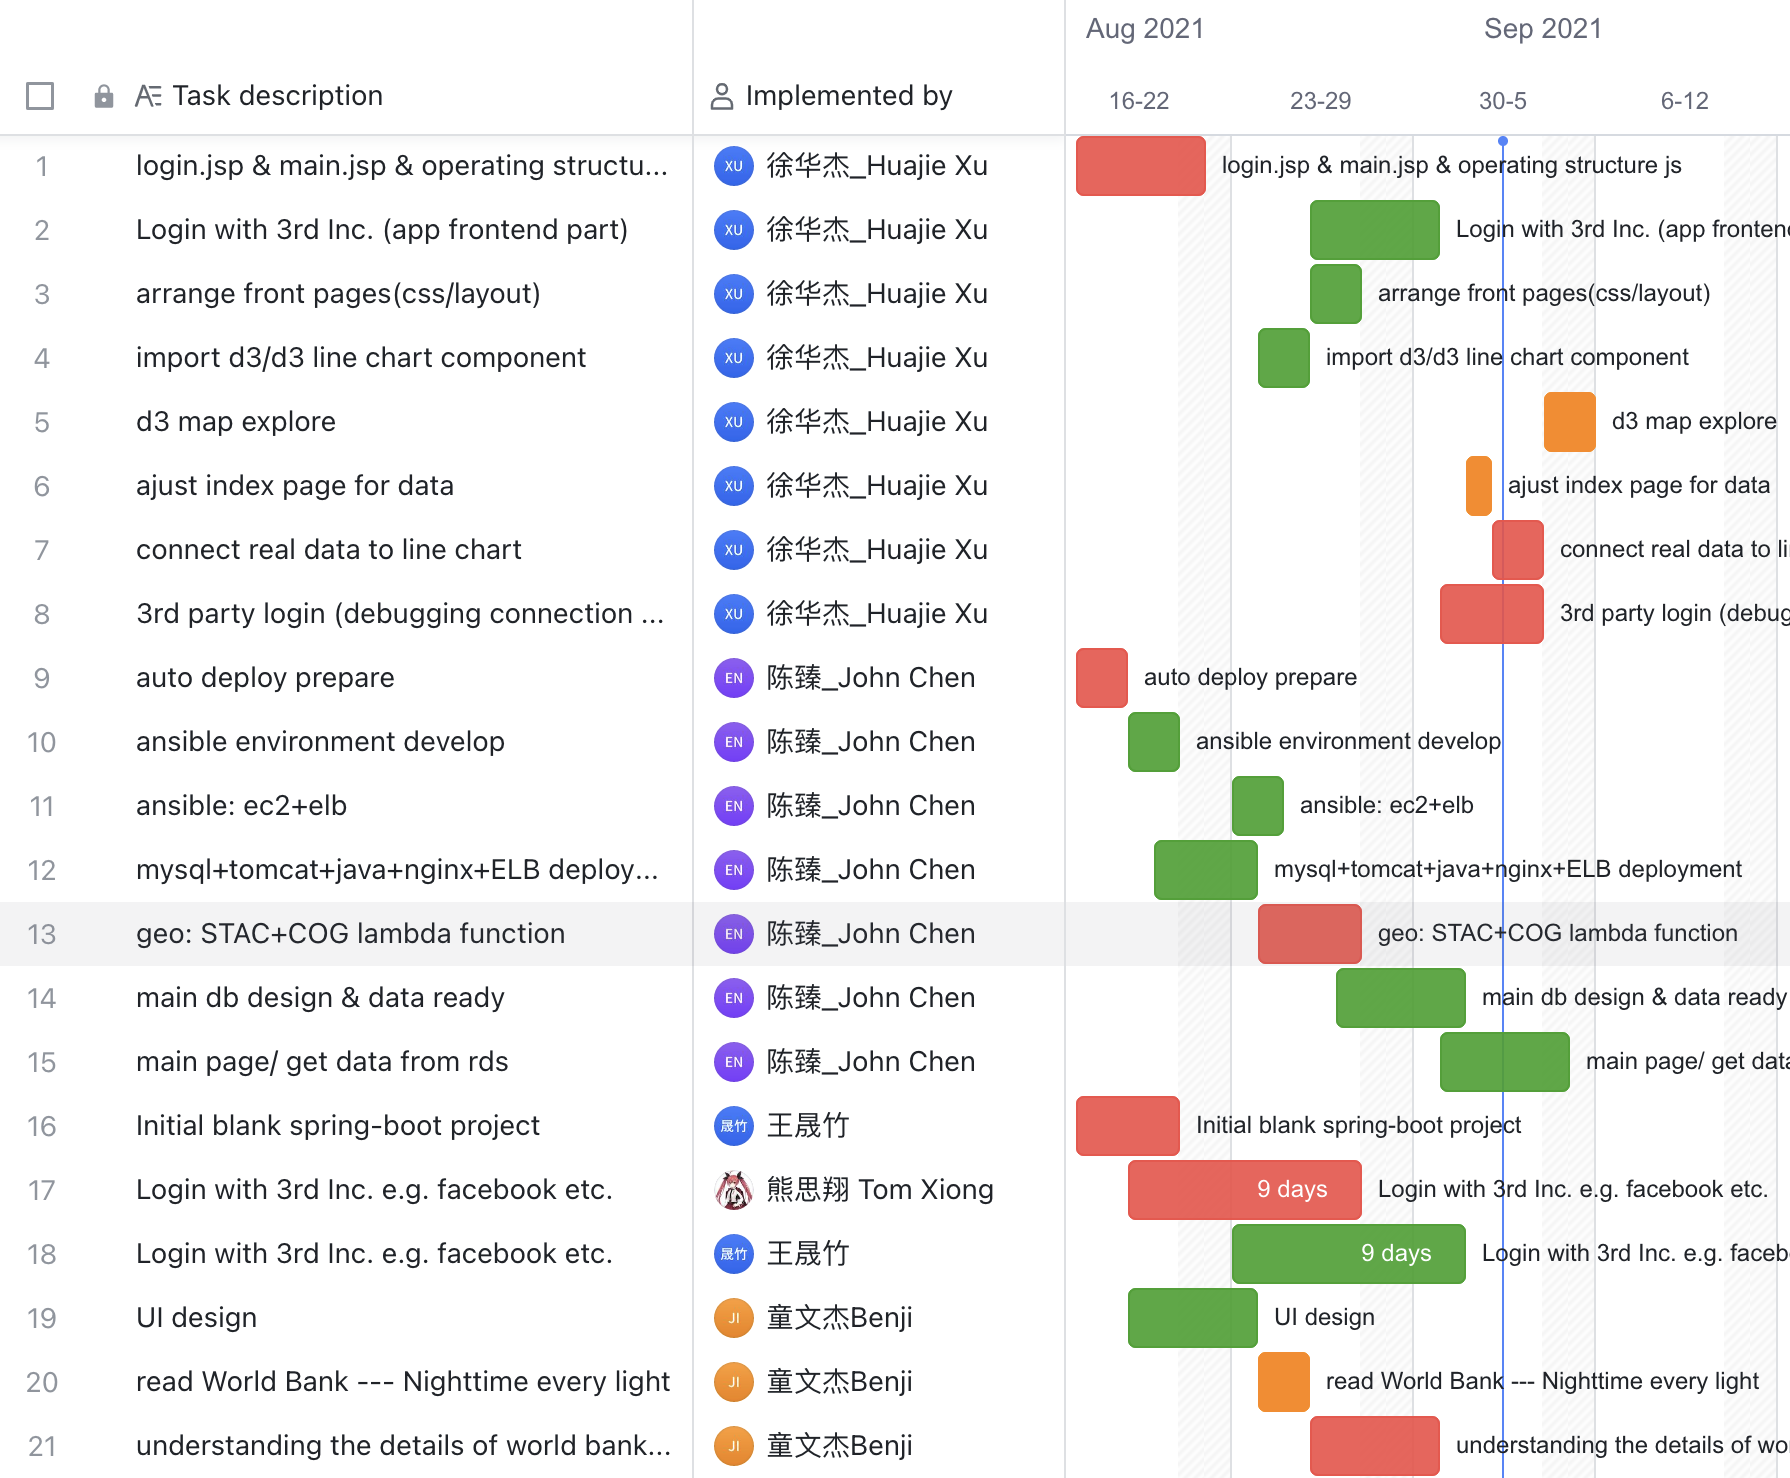
\includegraphics[width=260pt]{images/plan.png}}
    \caption{Project schedule}
    \label{fig1}
\end{figure}



The architecture of our solution is shown as Fig.~\ref{fig2}. Both security and budget are important, network address translation (NAT) gateway 
was used for essential network design. However, after two days, NAT had to close because of the budget alert. It is still necessary to hide the 
internal services into the internal network instead of exposing them to the internet.

There are two important methods to keep the password safely. The first one is IAM role. IAM role provides good security protection in the whole structure.
Different IAM roles are generated to attach to different Lambda functions. The execution roles are granted permission of access to necessary AWS services. 
There are some common policies for them, e.g. AWSLambdaBasicExecutionRole and AmazonS3FullAccess policies. The second one is Secrets Manager service in AWS.
All of the passwords in this project are stored in it. Visiting it through Secrets Manager when needed.


\begin{figure}[htbp]
    \centerline{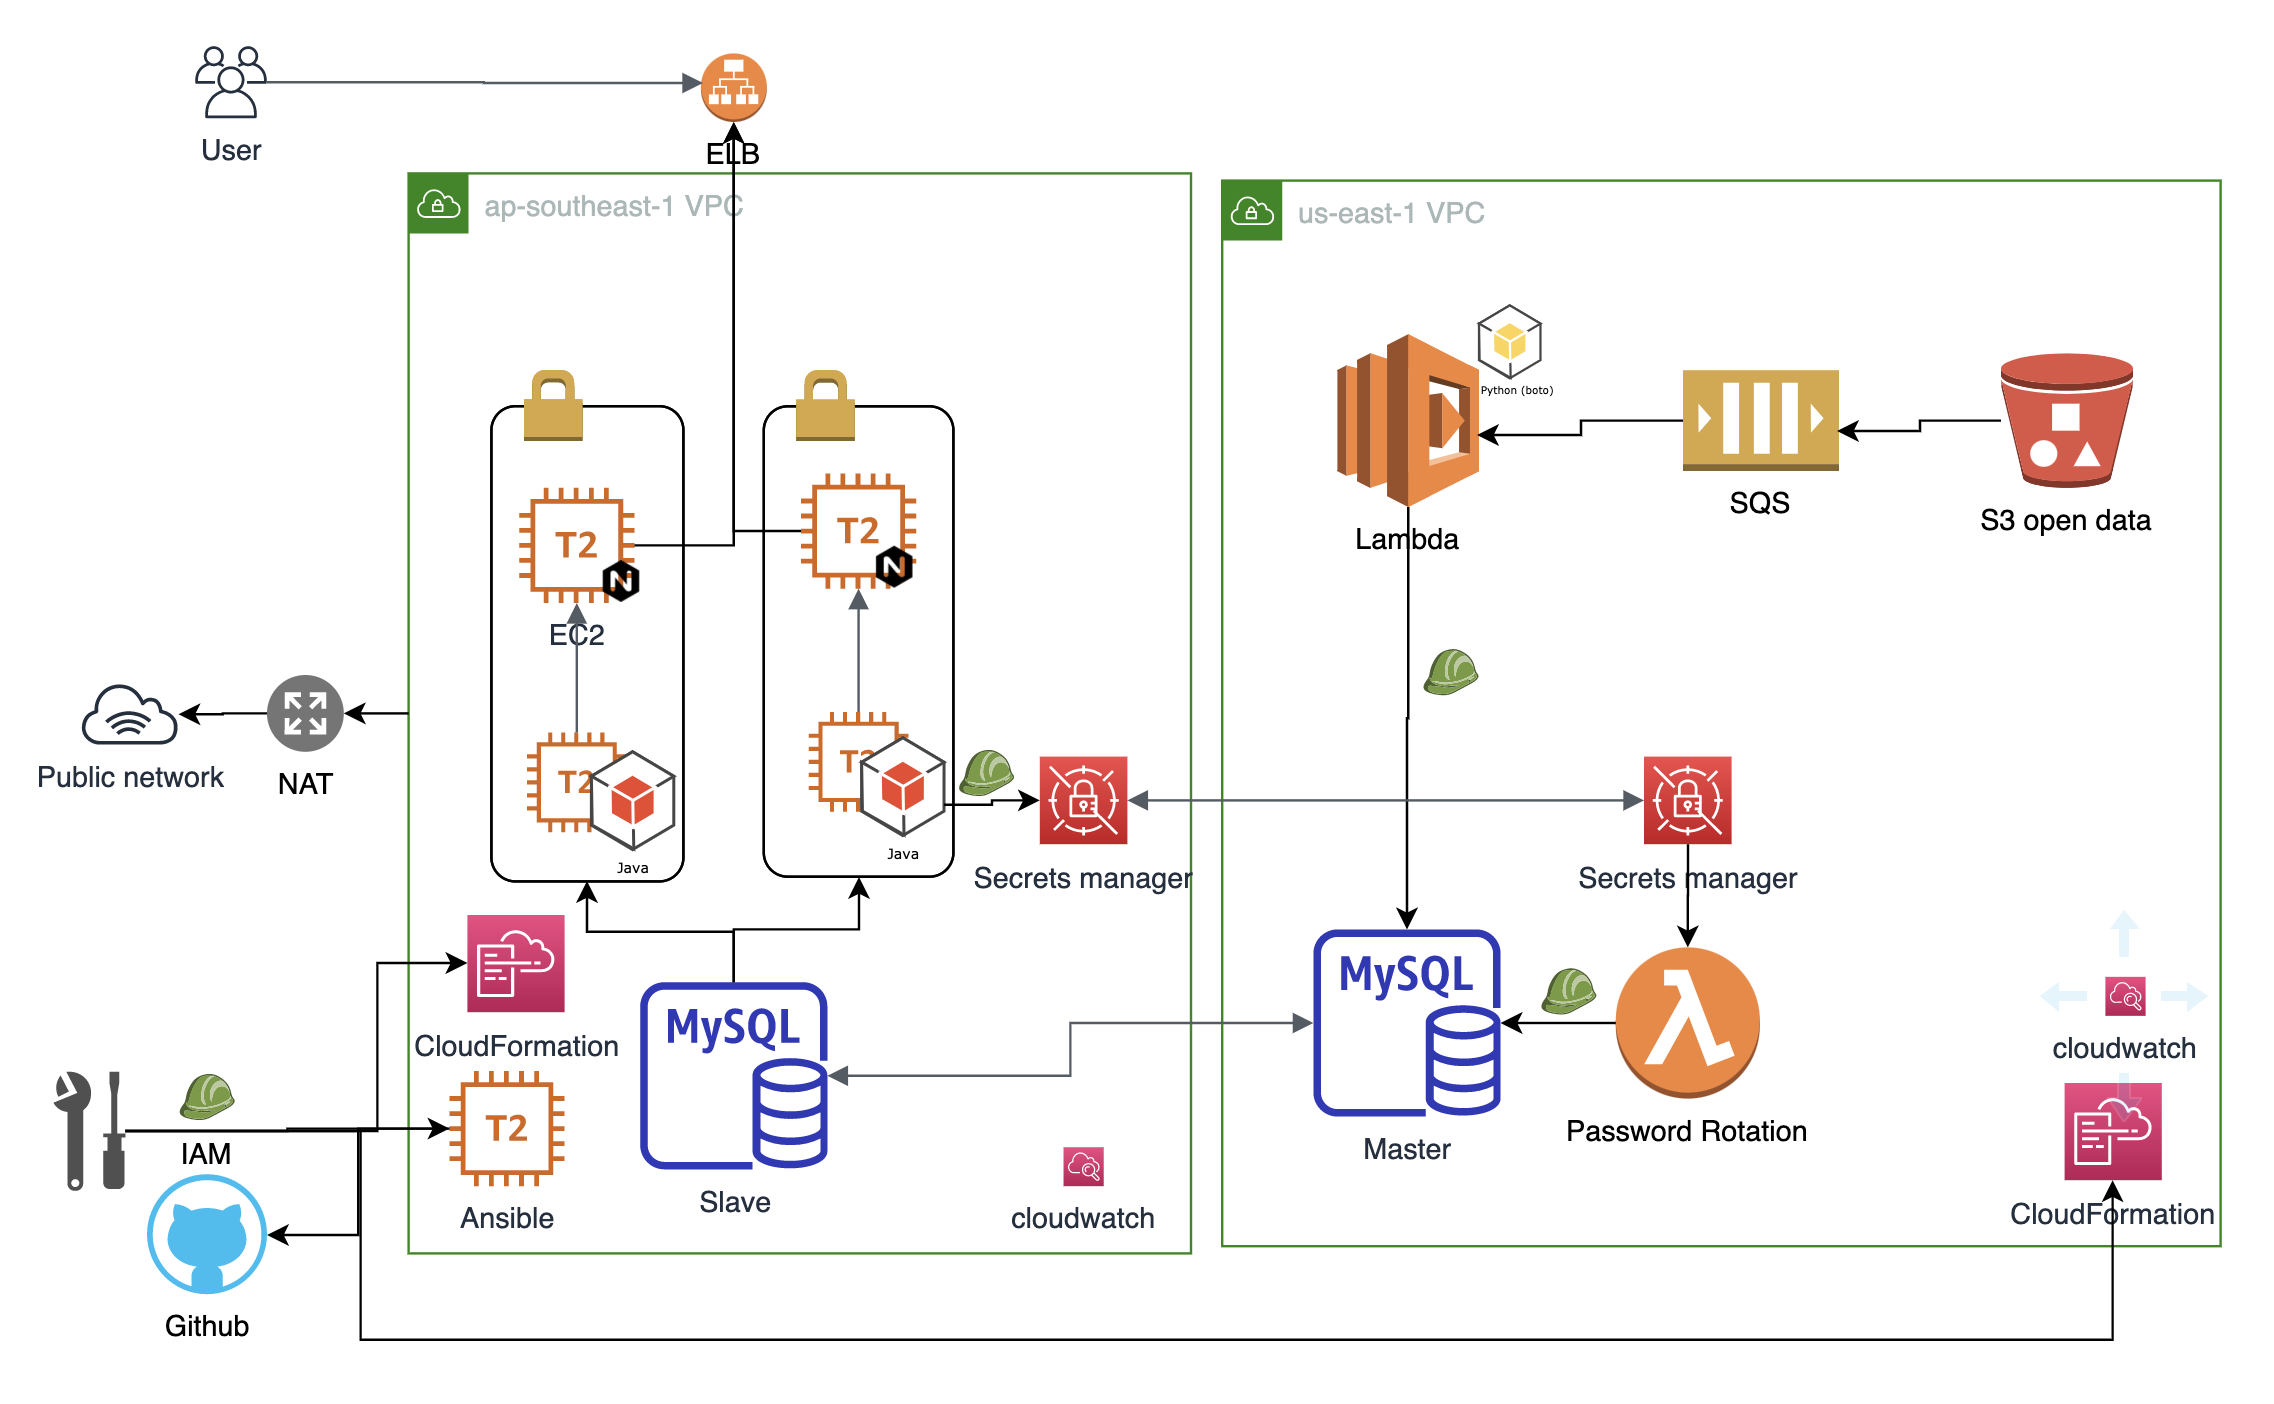
\includegraphics[width=260pt]{images/arch.png}}
    \caption{Architecture}
    \label{fig2}
\end{figure}
    
To process the S3 data, two Lambda functions are generated. One is to follow the STAC protocol to find the imagery, and another is to analyse pictures by GDAL, 
which is a kind of high cost computation in AWS. There are more than 4 pictures per day per area, and about 5,000 pictures per month totally. All the results processed by 
Lambda are stored in RDS and synced from us-east-1 region to ap-southeast-1 region. In addition, the password of MySQL is generated by a Lambda function and rotated 
timely. Therefore, the development team does not need to copy the password. Any features with passwords have to get it from Secrets Manager. 

When it comes to showing the result in ap-southeast-1 region, network security is the most essential thing because this part of service can be touched by end users. 
So except ELB and the deployment server, there are not any other servers with public IP. All the EC2 instances can visit public networks from the NAT, but public networks 
can not visit them directly.

To explain more steps, there are some summaries as below. 

\subsection{Overview of World Bank Light Every Night}
World Bank Light Every Night \cite{WorldBan13:online} is an integrated data collection center and data repository established by the World Bank in cooperation with the National Oceanic and Atmospheric Administration (NOAA) and the University of Michigan. It contains light collected at night. Satellite imagery for the past 30 years. So far, two sensors have been in use: the first is called DMSP-OLS, and its data collection is from 1992 to 2017. The other is called VIIRS-DNB, and its main data collection period is 2012-2020.
    
Both DMSP-OLS and VIIRS-DNB sensors use different wavelengths on the satellite to collect various light sources on the earth as optical data. These light source data mainly include brightness data generated by various human activities. Most of the light comes from cities, fishing boats, fires, or other natural light. It is a long process for the continuous light source data to be collected and stored. However, most of the basic data comes from the NOAA National Environmental Information Center (NCEI). Finally, all the data will be provided to the public as a shared database for analysis and use.
    
After continuous exploration, development, updates and upgrades, the University of Michigan supports cloud-optimized access to GeoTIFF format (COG) files through additional processing, and uses the Spatio-temporal Asset Catalog (STAC) standard to edit data for sharing. File and data sharing are ready. Continuously improving standards promote the integration of data and the integrity of the shared ecosystem, which is improving access to geospatial data sets, making them more widely accepted by the public, and making it easier to discover, process, and analyze geospatial data. Our project data will also use cloud-optimized GeoTIFF format (COG) and STAC standards to implement network-level applications.

\subsection{Remote sensing}
Research conducted by NASA shows that modern remote sensing technology was invented by the inspiration of cameras for more than 150 years\cite{earthdata28:online}. The first original photo appeared in the form of a "still image", but it inspired the idea and practice of people taking pictures and looking down on the surface of the earth. This idea appeared in the 1840s. The first photo was used for topographic mapping. At the end of the First World War, the cameras installed on the aircraft provided a bird's-eye view of a considerable area and provided a large amount of terrain data for military activities. After continuous research and development, the current remote sensing technology has reached a qualitative leap.

Remote sensing technology is usually used to describe objects, without direct contact, only to identify, observe and measure. Most of the data collected in this project are generated by the reflection or emission of objects or materials. These differences in wavelength or degree of radiation will also have different effects on the detection and measurement data. So through the collection of radiation and wavelength, analysis plus consideration of objects, types, density, and various aspects\cite{earthdata28:online}Finally determine the wavelength of the light to image.

\subsubsection{Orbits} 
Here are the 3 most commonly used orbits used to observe the changes of the earth and data collection, polar orbiting satellites, low-Earth orbit, and geostationary. More explanations and details will be elaborated below:

\paragraph{Polar and non-polar}
    
Polar orbiting satellites (picture ~\ref{satellites}) have an orbit close to 90 degrees to the equator. This angle allows the satellite to better perceive and observe the earth, so that more data can be collected more simply and in detail. Including polar regions and some areas where it is difficult to collect data\cite{WhatisRe36:online}. Most of the NOAA polar satellites mentioned in the project provide infrared and visible light earth image data. Sometimes they also collect some data on the atmosphere\cite{side357:online}. Most polar-orbiting satellites are sun-synchronous. This is to allow the satellites to pass the same position at the same solar time in each cycle. Such satellites will also reach the Antarctic and North Pole in different orbits to collect meteorological, ocean, land, climate and other professional data.

\begin{figure}[htbp]
    \centerline{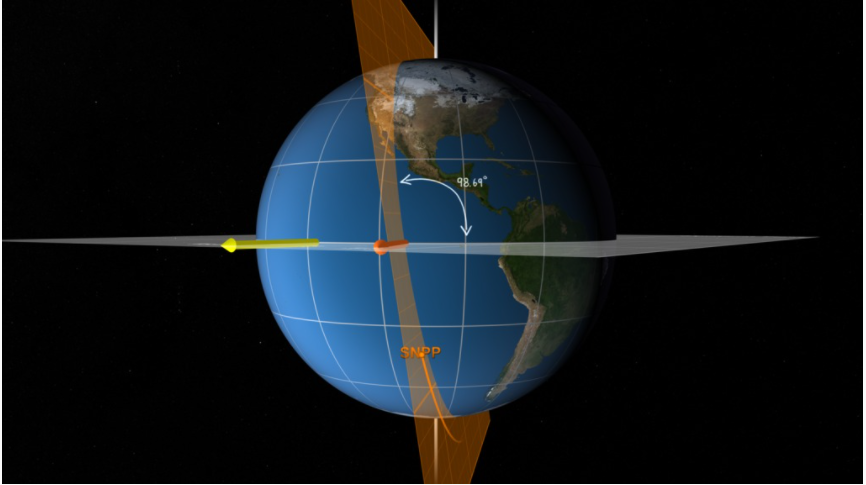
\includegraphics[width=260pt]{images/1.1.1.png}}
    \caption{Polar-orbiting satellites}
    \label{satellites}
\end{figure}
 
\paragraph{Low-Earth orbit}

Low Earth Orbit (LEO) (picture ~\ref{LEO}) is the closest orbit to the earth for a satellite. It is only less than 400 kilometers above the surface of the earth, but it may be even higher than 2000 kilometers. Range \cite{WhatisRe36:online}. Such low-orbit operation has inherent advantages for satellites in shooting satellite maps and navigation, etc. \cite{earthdata28:online}. The current high-resolution images are basically taken by it, and such orbits are often used by the International Space Station (ISS) as a common orbit. The design of this orbit makes it easier for astronauts to travel to and from it. The satellite in this orbit moves at a speed of about 7.8 kilometers per second; for a low-orbit satellite, it usually orbits the earth at this speed for only 90 minutes, which means 16 orbits around the earth. It provides good feasibility for the realization of satellite map technology and satellite positioning technology\cite{ESAkerne12:online}.

\begin{figure}[htbp]
    \centerline{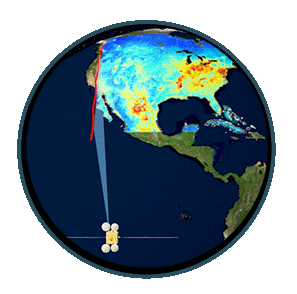
\includegraphics[width=260pt]{images/1.1.2.png}}
    \caption{Low Earth Orbit}
    \label{LEO}
\end{figure}


\paragraph{Geostationary}
The geostationary satellite's orbit (picture ~\ref{Geostationary}) can only be achieved at an altitude close to 35786 kilometers, and such satellites need to be detected at a fixed equatorial latitude\cite{Synchron89:online}. Such a satellite will be a place far away from the earth to observe and collect data. At the same time, it will be able to cover an area on the earth for a long time and continuously because of its location. For example, a weather satellite will operate in such an orbit. \Cite{WhatisRe36:online}. As far as the earth is concerned, the satellite operating in this way is stationary, its trajectory is synchronized with the earth, and its rotation period is also synchronized with the earth\cite{CelesTra70:online}.

\begin{figure}[htbp]
    \centerline{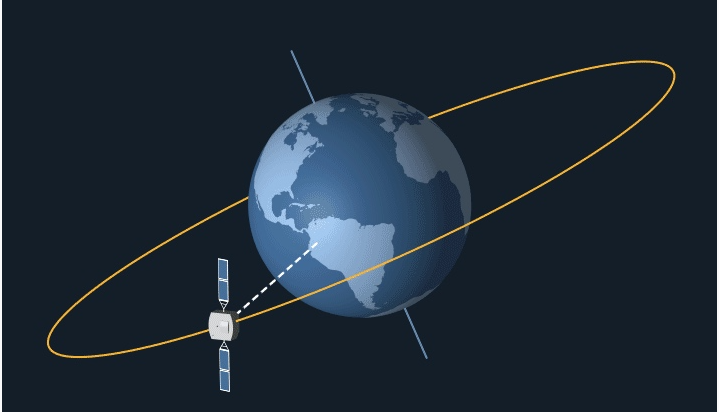
\includegraphics[width=260pt]{images/1.1.3.png}}
    \caption{Geostationary}
    \label{Geostationary}
\end{figure}

\paragraph{Electromagnetic Spectrum} 
The electromagnetic spectrum (picture ~\ref{Spectrum}) is a picture \cite{electrom75:online}. According to the frequency or wavelength distribution of electronic signals. These electronic frequencies or waves all travel at the speed of light in vacuum, but their frequencies, wavelengths, and photon energies are all different and have a wide range. The entire electromagnetic spectrum is divided into 7 types, radio waves, infrared radiation, visible light, ultraviolet radiation, X-rays and gamma rays. For gamma rays, it is still relatively far away from people in reality, so we will not discuss them. Therefore, the following part will give an introduction to the different emission, transmission and absorption of different waves, as well as their different practicability and scope of application, so as to have a better understanding of our project.

\begin{figure}[htbp]
    \centerline{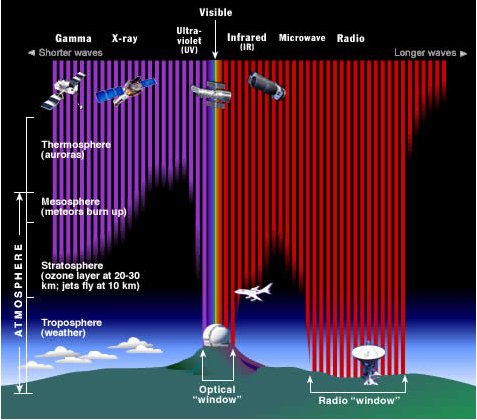
\includegraphics[width=260pt]{images/1.2.png}}
    \caption{Electromagnetic Spectrum}
    \label{Spectrum}
\end{figure}

\subparagraph{Radio}
    
Very Low Frequency (VLF): ELF is extremely low frequency and extremely low frequency, and its frequency is in the range of 
300 Hz to 30 kHz. It is a kind of radio wave, just like AM/FM signal, but with a lower frequency. It is very useful because 
it is mainly reflected at a height of 60-90 kilometers in the D zone of the earth's ionosphere, so it is effectively guided 
to a global distance in the earth's ionospheric waveguide. It is widely used to set up radio receivers almost anywhere on 
the earth \cite{Introduc19:online}. This signal can receive short radiation from lightning strikes in half of the earth.
    
Low Frequency (LF): Low frequency refers to the radio frequency in the range of 30 kHz–300 kHz \cite{httpswww63:online}. Low\-frequency AM broadcasting services are widely used in Northern Europe, North Africa, and Asia. In the current era, its main uses are aircraft beacons, navigation, information, and weather systems. 
    
Medium Frequency (MF): Medium Frequency means radio frequency (RF) in the range of 300 kHz to 3000 kHz \cite{httpswww49:online}. For example, 
the AM broadcast band is a medium wave (MW), and the MF band is also called the 100-meter band, which ranges from 100 
to 1000 hundred meters.
    
High frequency (HF): The wave frequency of the high frequency electromagnetic field is between 300 MHz and 3 GHz, and the wavelength is 1 m to 10 cm \cite{Highfreq56:online}. High-frequency electromagnetic fields do not occur in nature, so these electromagnetic fields are mainly man-made. With the rapid development of technology, among wireless technologies, high-frequency waves are more widely used, such as high-frequency communication. Such technologies can achieve the same call effect as satellites or telephones\cite{WhatisHi8:online}.

\subparagraph{Microwave}
    
Very high frequency (VHF) is ITU's electromagnetic wave in the range of 30 to 300 megahertz (MHz), and the corresponding 
wavelength is ten meters to one meter \cite{Veryhigh48:online}.
    
Ultra high frequency (UHF) has a wave frequency between 300 MHz and 3 GHz because the wavelength ranges from one meter to one tenth of a meter\cite{Ultrahig37:online}. Such UHF radio waves mainly propagate through the line of sight; however, they can be blocked by objects resulting in limited transmission capacity, so they are usually used for air traffic control air-to-ground voice communication or other transmissions such as TV broadcasts, WIFI, and walkie-talkies. Data dissemination and information communication\cite{UltraHig10:online}.
    
The wave frequency range of super high frequency (SHF) is 3 to 30 GHz \cite{Superhig8:online}. This frequency is also called the microwave frequency band. In this frequency range, many technologies have been invented, such as microwave oven technology, radar technology, wireless network technology, satellite communication technology, etc. Their realization and development are all related to wave frequency research. relation. These studies also provide people with great convenience and efficient quality of life.
    
Extremely high frequency (EHF) is a radio frequency in the electromagnetic spectrum from 30 to 300 GHz. It is a frequency between the ultra-high frequency band and the far-infrared frequency band. The wavelength of this radio wave band ranges from ten millimeters to one millimeter, so it is also called the millimeter wave band\cite{Extremel31:online}. Its transmission will be hindered by the atmosphere, so its transmission and rebroadcasting distance is very short, which also reduces its usability. This has also become the main obstacle to its development and use.

\subparagraph{Infrared}
    
Infrared radiation (IR) is a kind of radiant energy and electromagnetic radiation, which is invisible to humans, but we can 
still feel it. It occurs when atoms absorb and release energy with frequent fluctuations. All objects in the universe emit a 
certain degree of infrared radiation, such as the sun, fire, and the emergence of thermal imaging technologies are the research 
results of infrared technology \cite{L40416:online}.

\subparagraph{Visible}
    
The visible spectrum is the part of the electromagnetic spectrum that the human eye can see, so it is also called the visible wave. For such a wave, its wavelength is usually between 380 and 700 nanometers. The rainbow is a kind of light wave in space. There are seven colors. Because each color is different, their wavelengths are also different.Violet has the shortest wavelength. About 380 nanometers, the longest red wavelength, about 700 nanometers\cite{Vis73:online}.
 
\subparagraph{Ultraviolet}
    
UV light is in the electromagnetic spectrum between visible and X-rays, and its wavelength is between 400 and 10 nanometers \cite{uvlight14:online}. Among the ultraviolet light, red light has the longest wavelength, while violet light has the shortest wavelength. Therefore, the longer wavelength is called ultraviolet light, and the shorter wavelength is called ultraviolet light. Nowadays, the use of ultraviolet light can be seen everywhere, such as the invention of the currency detector, and the medical application of ultraviolet light shows its value.

\subparagraph{X\-ray}
    
X\ ray is a penetrating form of high-energy electromagnetic radiation. The wavelength range of most X\ rays is 10 picometers to 10 nanometers, the corresponding frequency range is 30 THz to 30 Hz, and the energy range is 124 eV to 124 keV \cite{XrayWiki61:online}. X-rays are also used for physical examination and diagnosis in modern medicine because of X-ray imaging technology. When the light beam passes through the body, different shades of bone, metal, or other materials will be formed due to the different density of the material, thus forming an image \cite{XrayImag8:online}.

\subsection{Spatial, spectral, and temporal resolutions in remote sensing}
    
\paragraph{Spatial resolution} 
    
In remote sensing, the spatial resolution shows the smallest possible feature that a satellite image can display, which means 
that the size of a pixel on the ground constitutes the smallest "point" of an optical satellite image. If the satellite tries 
to capture the size of the scene 700KM from the earth (300m x 300m), the imaged pixels will be very low and the image will become 
very blurry \cite{AtlasAIW26:online}. The spatial resolution is divided into 3 levels:
    
    \begin{itemize}
        \item Low resolution(LR): over 60m pixel 
        \item Medium resolution(MR): 10 ‒ 30m pixel 
        \item High resolution(HR) ‒ ultra-high resolution(UR): 30cm ‒ 5m pixel
    \end{itemize}
    
Not many details about the capture are determined by the pixels of the spatial resolution. If improvements are made to obtain 
more captured details, a large number of cameras will be required to achieve detailed scenes. For the same purpose, space scientists 
need to use a single-pixel to represent the linear dimension on the ground, where the difference in pixels and colors will be 
recommended for measurements on the earth according to the satellite's use and coding method. In the 1980s, NASA satellite data from 
Landsat had 60 million pixels at the time, but with the advancement of the times and the rapid development of technology, 60 million 
pixels have become less leading. The current highest resolution satellites can provide 30 cm accurate imaging \cite{Satellit48:online}. 

\paragraph{Spectral resolution} 
    
The International Commission on Illumination (CIE) organization defines the light response of human vision as the range of 380nm to 
780nm and provides a weight table so that the public can use the instrument to study the measured value at the wavelength multiplied 
by the corresponding human vision \cite{spectral41:online}. These tables are provided at intervals of 1 nanometer, 5 nanometers, 
and 10 nanometers. Resolution refers to how many data points are used in the calculation of the image. For the spectral resolution, 
it is to define the measurement point in the spectral result one step further.

\paragraph{Temporal resolution} 
    
Time resolution refers to the repetitive period or frequency surface of the sensor revisiting the same part of the earth. Think of it as the time to take multiple measurements of the cross section and then reconstruct the image. This time is also called the "revisit time" of the satellite.For example, the greater the stripe width of a polar-orbiting satellite, it is regarded as the width of the sensor's "cross-orbit" field of view during the passage of the orbit, and 
the higher the resolution time \cite{Topic43:online}.


\subsection{Vue}

Vue is a progressive framework, which is perfectly capable of powering sophisticated Single-Page Applications when used 
in combination with modern tooling and supporting libraries \cite{Introduc89:online}. In fact, Vue is used for two main reasons. Firstly, 
with Vue, the server-side code can be effectively decoupled from the front-end UI which means back-end and front-end 
teams can focus on doing their jobs. And second one is because all members of our group are inexperienced in constructing 
front-end. Therefore, the front-end framework we need should be easy to get started and has a straight forward learning 
curve, which is one of Vue’s characteristic. That is also why these years saw its hot upward trend in GitHub stars number.

\subsection{D3}

Fundamentally, D3 is a JavaScript library for creating data visualizations, an elegant piece of software that facilitates 
generation and manipulation of web documents with data \cite{2013Interactive}. Our solution can demonstrate potential business 
value only if all the data processed by Lambda can be vividly presented to users. By the way, it can be easily imported to 
Vue because they all base on JavaScript.
 
\subsection{Spring-boot}

Spring-boot is a Java web framework that can help developers build their web instance very quickly. It is easy to build a 
stand-alone, production-grade application by it \cite{SpringBo66:online}. Because of its features such as no code generation 
and no requirement for XML configuration, it is the best choice for a Java development team.

\subsection{Ansible}

Ansible is a famous open source deployment platform, which is convenient to enable the infrastructure as code (IaC). 
It is the main tool to deploy most of the services in this project. In particular, a single EC2 instance with the public 
IP is provided for it. But AWS service has to provision services by aws-cli instead of Ansible itself. There are still 
some libraries providing these functions but mostly are from the external part.

\subsection{CloudFormation}

CloudFormation is a service in AWS, which can organize services very quickly and configure them by Yaml or Json. There are
several templates for provisioning different services. It is more convenient than Ansible for some services. In this project, 
RDS and Lambda Services are dependent on it.

\subsection{Nginx/Tomcat}

Nginx is a widely used web server all over the world. It also has excellent performance as a reverse proxy. 
Fontend server plays a role in this project. Tomcat, which is behind Nginx, is a traditional Java web container supporting 
Java Servlet. The visualisation is designed by Java and runs in this container. Both Nginx and Tomcat are well-known because of 
the open source community and internet companies choosing.

\subsection{RDS/Lambda/Secrets Manager/SQS/EC2/NAT}

These items are the names of services on AWS. In particular, Lambda is used to generate temporary passwords of RDS, and store it in 
Secrets Manager. It is really a good method to enhance the security for the password of database. On the other hand, NAT is a 
good feature for isolating the internal and external networks, but the price is too high to be used all the time in this project.

\subsection{Oauth github}

GitHub's OAuth implementation supports standard authorization code type or OAuth2 device Authorization
for apps that do not have access to a web browser. If you want to skip authorizing your app in
standard method, for example, when testing app, you are able to apply the non-web application flow/
If you want to create an OAuth Application in GitHub, client will need to log into Github, visit
the Applications page under your organisation's settings, click Register 'New Application',
set HomePage URL: Enter the Quay Enterprise URL as the HomePage URL, finally, save your settings by
clicking the Register application button. An OAuth App could be used as an identity provider by enabling
a "Login with GitHub" as for the authenticated user. Do not build an OAuth app if you want your
application to act on a single repository. With the repo OAuth scope, OAuth apps is able to act on
all of the authenticated user's repositories. If you want to register for OAuth application,
in the upper-right corner of any page, click your profile photo, then click Setting, in the
left side bar, click Developer settings, in the left side bar, click OAuth Apps, click New
OAuth App, in Application Name, type the name of your app.OAuth is a standard that apps can
use to provide client applications with 'secure delegated access'. OAuth works over HTTPS and
authorizes devices, APIs, servers, and applications with access tokens rather than credentials,
such as your client ID, yout client secret key. Nowadays, OAuth2 is the most widely used form of
OAuth.

\section{Proposed solution}

A demo has finished all tasks following the plan on time in this project. But to save budget, stopping NAT and processing parts of data are 
the temporary approaches. It is also possible to deal with the cloud and other disruption to ensure the accurate radiance value. All the 
other details are described as below.

\subsection{Whole infrastructure and automatic deployment}

The main architecture is shown as Fig.~\ref{fig2}. First of all, two kinds of IaC platform, which are Ansible and CloudFormation, are used for deployment.
Ansible is the first choice that can be easily used in most situations. When some complicated services need to be configured, CloudFormation is 
better. Secondly, ELB is the only entrance to the project. That is the best practice for network security that can mitigate the effects 
of public cyberattacks. Thirdly, IAM roles are used at all kinds of important scenarios, for example, deployment, database visiting, various services visiting.

The source code of the entire demo was maintained on Github. The repository URL is https://github.com/A2Inc/A2. There are various languages in it including 
CSS, Vue, Java, JavaScript, Python, Tex. The contributions of the team on this demo are shown on Github as Fig.~\ref{fig3}.

\begin{figure}[htbp]
    \centerline{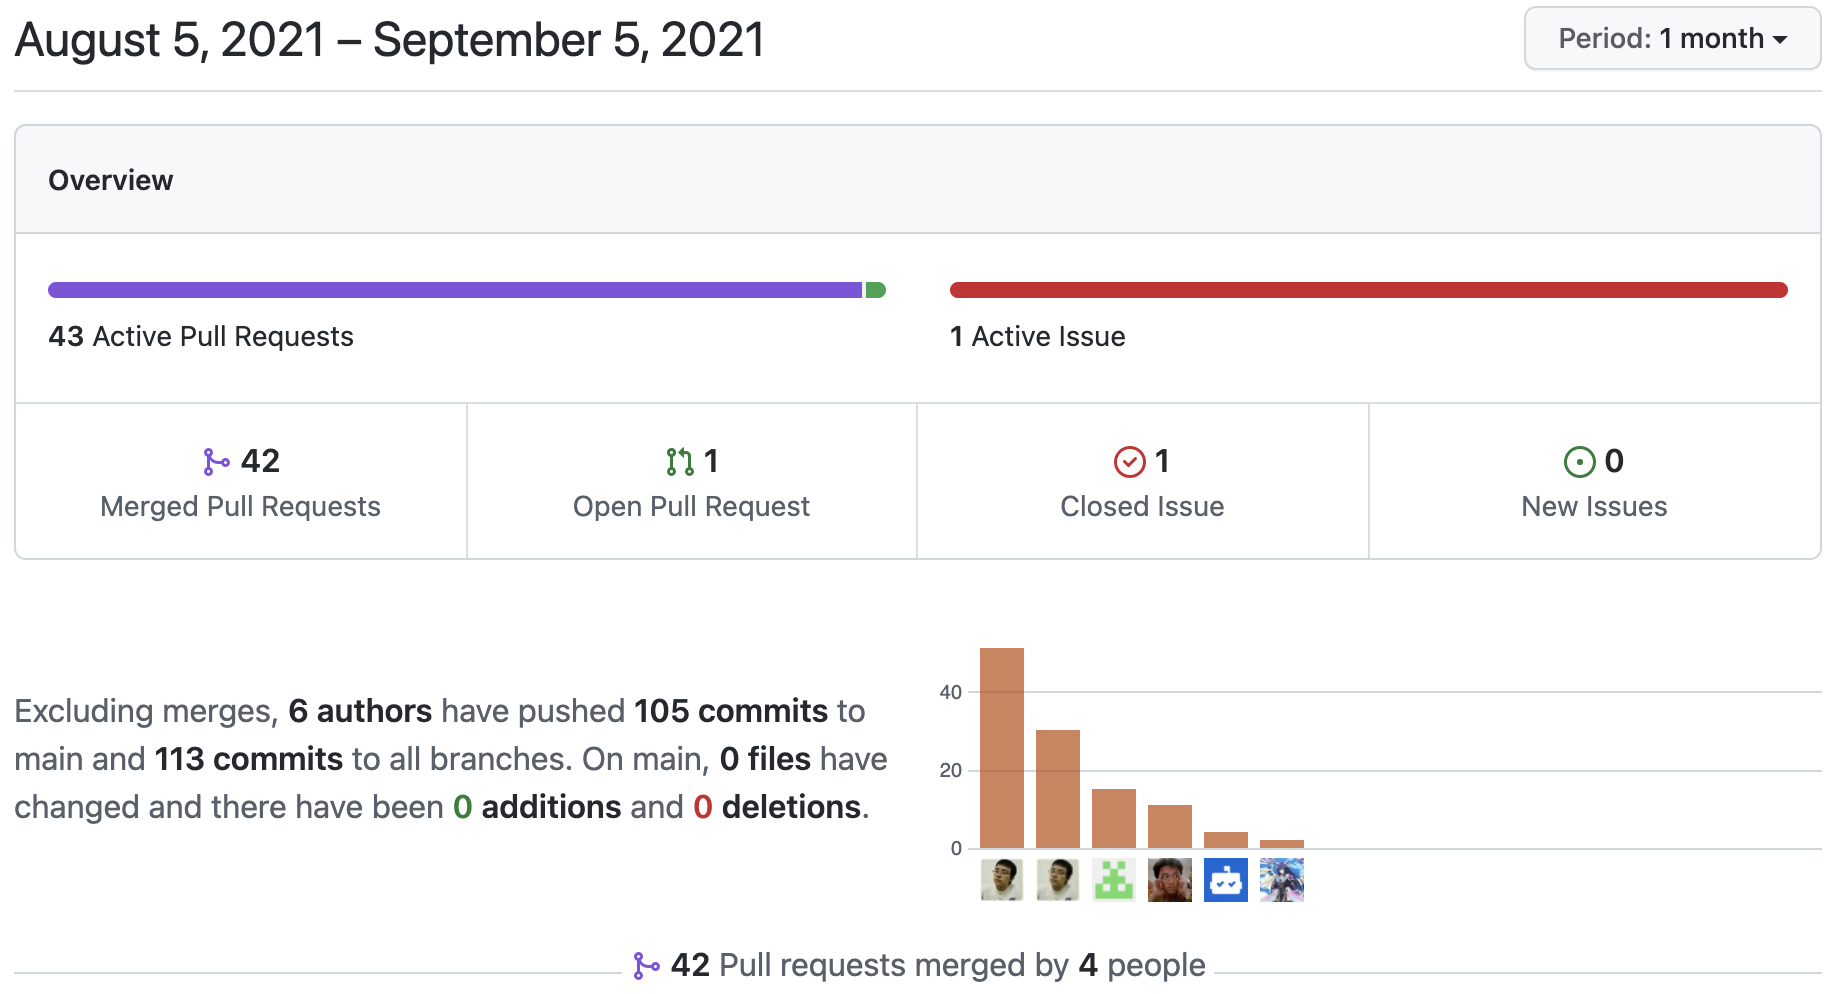
\includegraphics[width=260pt]{images/github.png}}
    \caption{Overview of Github}
    \label{fig3}
\end{figure}

Java, Python and Vue are the relatively useful tools in this demo. The reason for choosing Java is that almost all of the team members have been good at it. Python 
has a lot of library processing images. It is, therefore, the best choice for geographical imagery. Vue has powerful frontend capabilities. It is also the best for a 
visualisation demo. Latex is used to generate reports and slides.

To speed up the development of the demo, automatic deployment has been built from the first day. There are two types of deployment scripts. The first type is shown 
as Fig.~\ref{ansible}, which is built by Ansible. The entire basic environment can be built from this directory. Below steps can build a clean deployment for this demo.

\begin{itemize}
    \item Ensure that the local aws-cli configuration is ready to use, i.e running "aws configure".
    \item Run "ansible-playbook -v -i hosts2 supervisor.yml" to generate a new EC2. Get the IP address.
    \item Run "ssh -i ~/.ssh/[key] root@[ip]" to login.
    \item Run "git clone https://github.com/A2/A2.git" to get the code.
    \item Install the basic requirements and initial part as the README.md under the "deploy" directory.
    \item When requirements are ready, run "ansible-playbook -v -i hosts site.yml" will deploy all of the services including Tomcat, Nginx, ELB, Java. 
\end{itemize}

\begin{figure}[htbp]
    \centerline{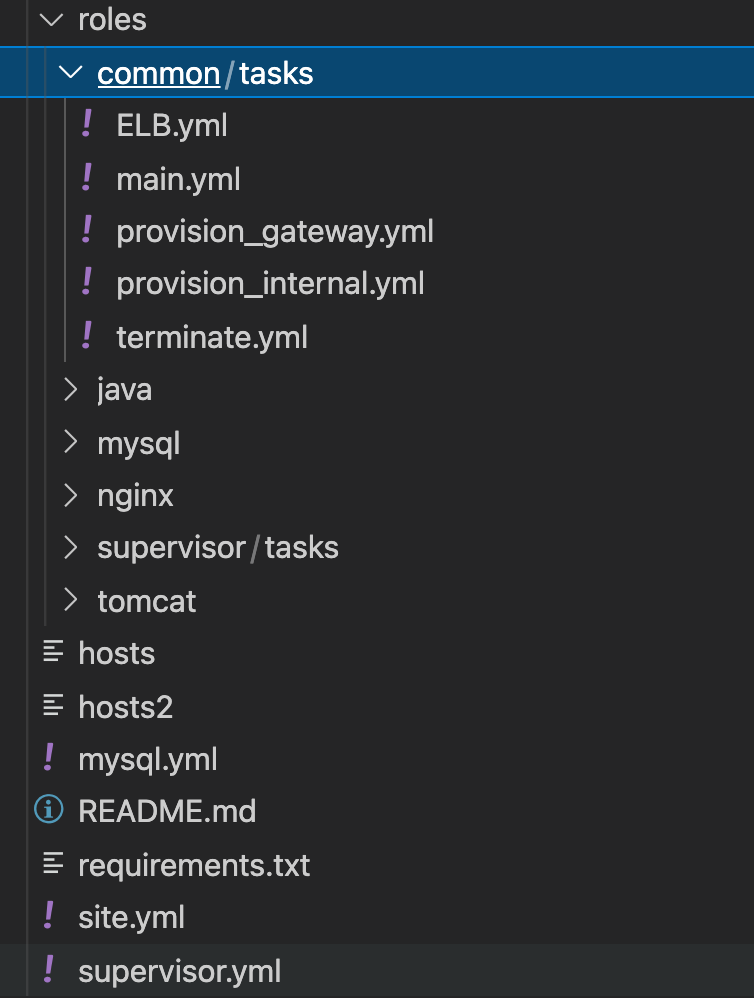
\includegraphics[width=260pt]{images/ansible.png}}
    \caption{Deployment By Ansible}
    \label{ansible}
\end{figure}

The second type of deployment is shown as Fig.~\ref{cf1}, which is built by CloudFormation. In Fig.~\ref{cf1}, there are CloudFormation configuration files. 
Running "make deploy" in this directory will follow the steps below to built the Lambda functions.

\begin{itemize}
    \item Generate a role named lmdRole and attach various access rights.
    \item Generate some SQS queue for the Lambda functions.
    \item Define the functions and bind the role, handlers, queues, configurations.
\end{itemize}

\begin{figure}[htbp]
    \centerline{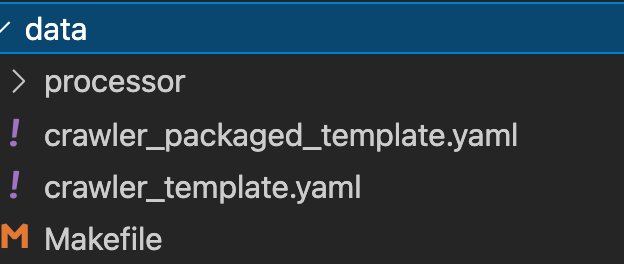
\includegraphics[width=260pt]{images/cf-1.png}}
    \caption{Deployment of imagery process}
    \label{cf1}
\end{figure}

Running "make deploy" in the directory shown as Fig.~\ref{cf2}, which is "A2/deploy/roles/mysql/templates", can create a slave RDS MySQL instance. Because 
a cross-region database replica is needed in this demo, running "make master" can build another master RDS MySQL after changing the aws-cli region. And the 
slave instance is replicated instantly from the master instance. Both of the commands for MySQL use CloudFormation. The first one is just a very 
simple process, but the second one is also generating a Lambda function to rotate the MySQL password in the master database, and store it in Secrets Manager service. 

\begin{figure}[htbp]
    \centerline{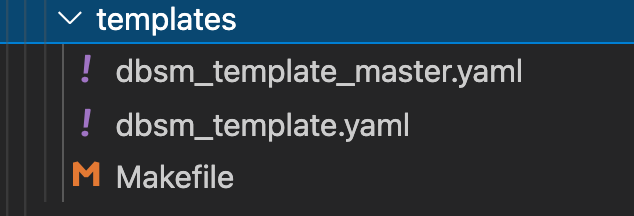
\includegraphics[width=260pt]{images/cf-2.png}}
    \caption{deployment of MySQL}
    \label{cf2}
\end{figure}

After the above steps, the entire demo should be ready for processing s3 imagery and users can visit it from the ELB URL.

\subsection{Frontend}

\subsubsection{Frontend construction}
 
\paragraph{NVM}
    
“NVM (Node Version Manager) is a version manager for node.js, designed to be installed per-user, and invoked per-shell” 
\cite{nvmshnvm87:online}. With it, it is possible to manage multiple versions of node.js in same machine.

\paragraph{NPM}

"NPM is the world's largest software registry. Open source developers from every continent use NPM to share and borrow packages, 
and many organizations use NPM to manage private development as well" \cite{Aboutnpm31:online}. Since NPM is the default package manager for the 
node.js, so Vue, webpack and other dependencies can be installed or uninstalled by it.

\paragraph{Native Vue or Webpack}

"At its core, webpack is a static module bundler for modern JavaScript applications. When webpack processes your application, it 
internally builds a dependency graph from one or more entry points and then combines every module your project needs into one or 
more bundles, which are static assets to serve your content from" \cite{Concepts28:online}. Not only Vue but also other frameworks like React, 
Angular depend on webpack to build boilerplates.

\paragraph{Vue cli}

"A simple CLI for scaffolding Vue.js \\projects" \cite{Introduc89:online}. With it, user can pull template from vuejs-templates and generate 
the basic webpack \+ Vue project.

\subsubsection{Frontend function}

There are two main tasks of frontend, third party login and data visualization.

\paragraph{Third party login}

At present, we have implemented third party login by GitHub. Frontend will redirect to GitHub webpage to let user get authenticated 
by GitHub to get assertion, which is practically a temporary code. Then frontend will provide this code to service provider, which 
is ELB in our solution, to exchange for token to complete whole authenticating process. All API are used securely according to official 
documents \cite{Authoriz26:online}.

Another issue that needs attention is how to keep access token in client-side because user may not want to jump to GitHub every time when signing in. However, whether storing the token in local storage or cookie, user data is both under threaten of XSS or CSRF attack. So, in this solution, there is a JSESSIONID encrypted and stored in cookie by server, which is the real proof to obtain service. Because it is generated by the server, using the “httpOnly” flag, so JavaScript cannot read it.

\paragraph{Data visualization}

For three specific research-\\ targeting areas, the data format is just like Fig.~\ref{dffg}. It is an array in which 
each element shows lots of details of one section of COG file at a particular time point. Because each time the section, also showed 
as “window” in the image, is different from each other, so directly comparing “radiance” of each element is meaningless. To show the 
level of night lights of different area, “radiance” divided by “pixels” is more valuable since it has nothing to do with the size of 
“window”.

\begin{figure}[htbp]
    \centerline{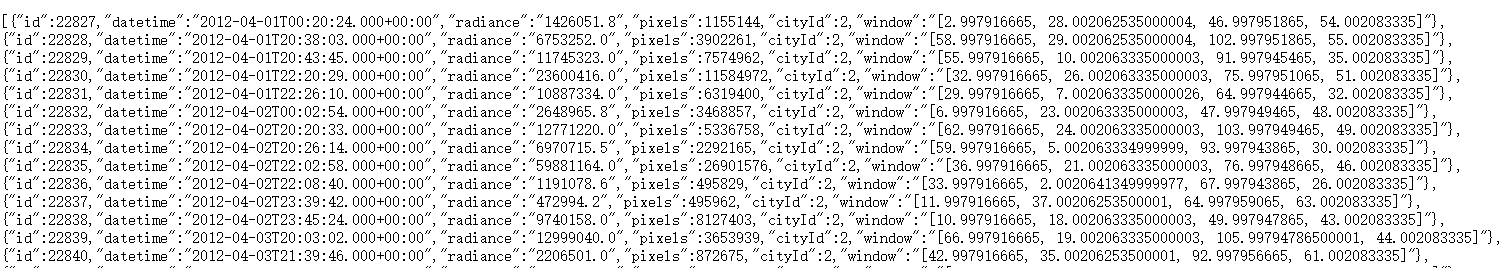
\includegraphics[width=260pt]{images/Data_format_frontend_get.png}}
    \caption{Data format}
    \label{dffg}
\end{figure}
 
Line chart as Fig.~\ref{lchart} is very suitable for showing the trend of a series of data changing over time. In order to provide more 
information, user can click the check buttons above the chart to see annual averages, monthly averages and daily averages of radiance 
per pixel.  

\begin{figure}[htbp]
    \centerline{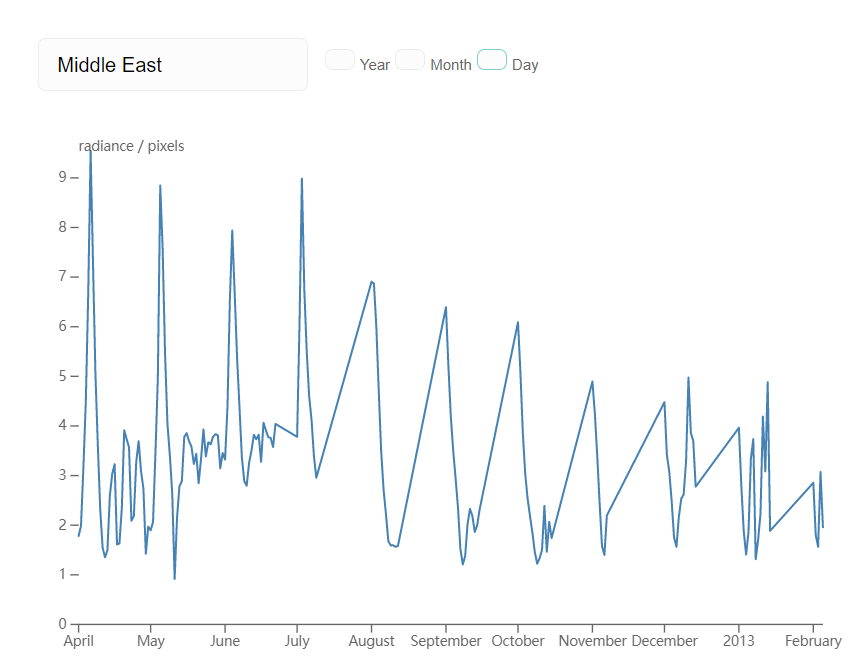
\includegraphics[width=260pt]{images/Line_chart.png}}
    \caption{Line chart}
    \label{lchart}
\end{figure}

Only relying on line chart cannot visually display all the information. Besides “radiance” and “pixels” there are still “window” representing the sampled area. Obviously, the most intuitive way to visualize area is using the map. In the map, the blue rectangles highlight the three researched areas, east of China, Middle East, and New Zealand as Fig.~\ref{wmap}.

\begin{figure}[htbp]
    \centerline{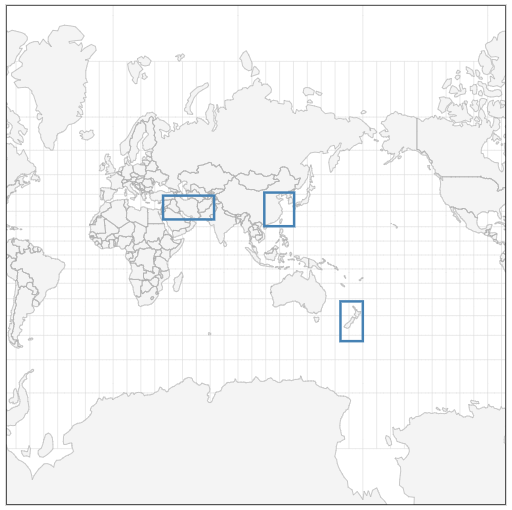
\includegraphics[width=260pt]{images/Worldmap.png}}
    \caption{World map}
    \label{wmap}
\end{figure}

Interaction is also important. User can hover the curser over points in line chart and the tooltip will pop up, showing the details, like the date and number of samples. Meanwhile, in the map, all the sampled areas will be highlighted by the red rectangles as shown in Fig.~\ref{iov}.

\begin{figure}[htbp]
    \centerline{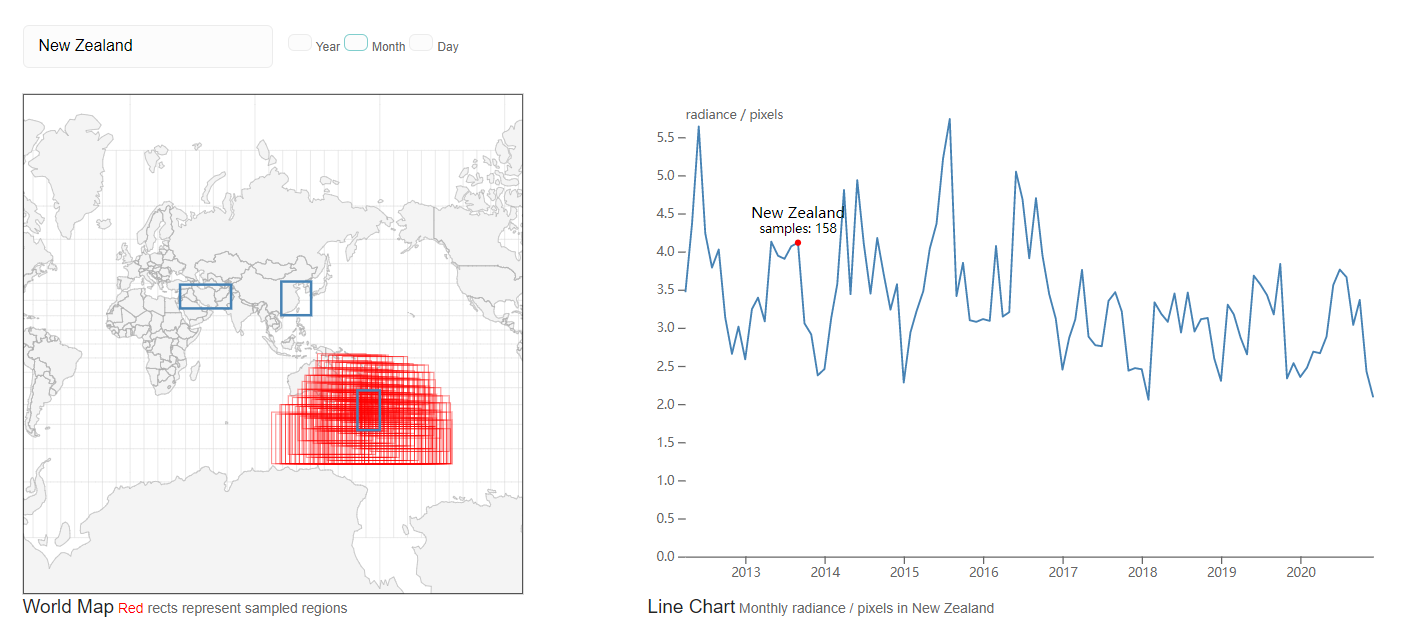
\includegraphics[width=260pt]{images/Interaction_of_visualization.png}}
    \caption{Interaction of visualization}
    \label{iov}
\end{figure}

\subsection{Login}
Springboot website adds third-party login Github login based on OAuth2
1. Introduction to OAuth2
OAuth is currently the most popular authorization mechanism used to authorize third-party applications and
obtain user data. OAuth has been widely used all over the world, and the current version 2.0. Simply put,
OAuth is an authorization mechanism. The owner of the data tells the system that they agree to authorize
third-party applications to enter the system and obtain these data. The system thus generates a short-term
entry token, which can be used in place of a password for use by third-party applications. Therefore.
the role of token and password is the same, both can enter the system, but these are three differences:
- The token is short-term, it will automatically expire when it expires and the user cannot modify it.
The password is generally valid for a long time and the user will not change if it is not modified.
- The token can be revoked by the data owner and will become invalid immidiately.
- The token has a scope, because the token has the same function as the password, the token must
also be kept strictly confidential. The consequences of leaking the token and leaking the password are
the same. This is why the validity period of the token is very short.
2. the principle of Github third-party login
Third-party login is actually OAuth authorization and authentication. The user wants to log into the
A website, and the A website allows the user to provide data from a third-party website to provide his
identity. Obtaining the identity data of a third-party website requires OAuth authorization.
Take the use of Github as a third-party login as an example:
The user clicks on the website to log in using Github, and the A website jumps to Github, callback
URI and Client ID will be brought:
1. Github asks the user to log in, and then asks "A website requires XX permmission, do you agree?"
For the same website, after agreeing once, user authorization is not required for logging in next time.
2. If the user agrees, Github will redirect back to website A and send back an authorization code.
3. A website uses the authorization code to request a token from Github.
4. Github returns the token.
5. Website A uses the token to request user data from Github.

\subsection{Imagery Overview}
The resource on AWS is the Light Every Night dataset of all VIIRS DNB and DMSP-OLS night satellite data. Its resource type is S3 Bucket on AWS cloud server. People can directly access files on Amazon cloud service through arn:aws:s3::globalnightlight, and its region is us-east-1\cite{WorldBan13:online}.

For implementing the web-level application, understanding the database of the Light Every Night dataset is essential 
for our team. Then I have accessed this dataset via the AWS instance Linux server. 

Under this path, there are three main types of folders, like-named by date (201204,201505…201603), named by satellites 
(F10, F12…F18), and named by npp\_date.

\subsubsection{DMSP-OLS}

DMSP is a series of polar-orbiting satellites of the US Air Force. The sensors on this model satellite were used in the 
initial design to observe weather-related indicators in the visible and infrared wavelength ranges during the day and night. 
DMSP satellites can be divided into "day/night" or "dawn/dusk" satellites according to their transit time. One side of the 
orbit of the day and night satellite images the dayside of the earth, and the other side images the night side. In 1992, when 
the digital archive began to be created, two DMSP satellites collected data and named them F10 and F11. F10 is in day/night 
orbit, F11 is in dawn/dusk. Since then, eight satellites have been launched, F12-F19, of which F12, F14, F15, F16, and F18 
were launched in day/night orbits.

This part DMSP-OLS data which are named from DMSP satellites as I mentioned before. The file name was generated from the 
satellite's name and year. Like F101992, which means the data was collected by satellite F10 in 1992. There are many files 
from 1992 to 2013 that can be used by the public.

\begin{figure}[htbp]
    \centerline{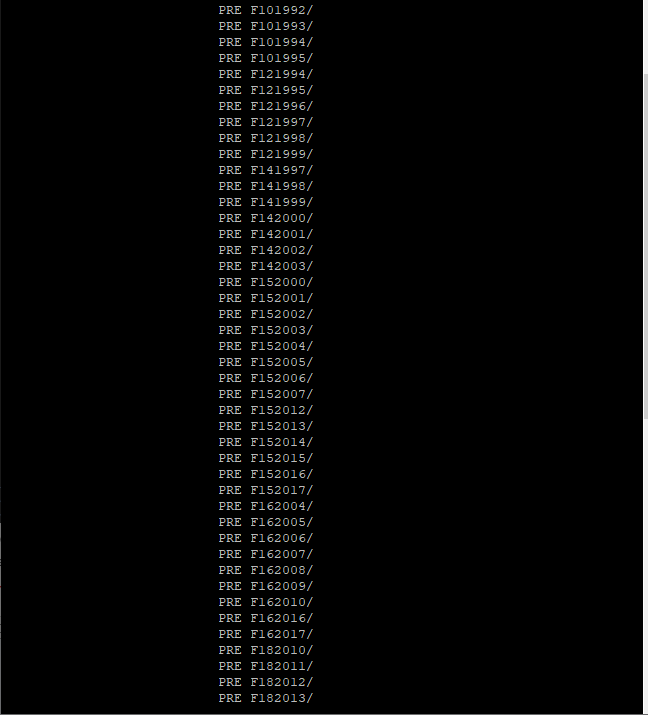
\includegraphics[width=260pt]{images/2.png}}
    \caption{folders}
    \label{folders}
\end{figure}

This picture (Fig.~\ref{folders}) is showing lots of folders of nighttime data.  In those folders, there are tons of .OIS files. 

For example: this is a file from database called \\F12199501010014.night.OIS, and lots of information will be given to this file.

\begin{itemize}
    \item F12 = satellite name
    \item 1995 = year at start of orbital segment 
    \item 01 = month at start of orbital segment 
    \item 01 = day of month at start of orbital segment 
    \item 00 = hour of day at start of orbital segment
    \item 14 = minute of hour at start of orbital segment 
    \item .night = orbit is cropped to only nighttime data 
    \item .OIS = acronym for OLS Interleaved Smooth
\end{itemize}


All those details about this file are giving more information for users to understand how the data be stored in the AWS database server. 

The satellite's timeline illustrates that the "F" satellites be used in different years.

\begin{figure}[htbp]
\centerline{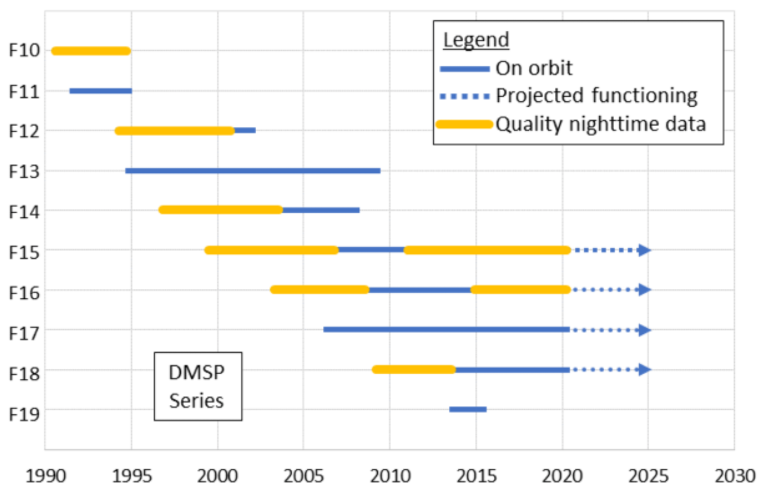
\includegraphics[width=260pt]{images/2.1.png}}
\caption{nighttime data}
\label{nighttimedata}
\end{figure}

The line chart demonstrates the different periods of how they are used in acquiring nighttime data.  It is clear to know F10 satellite 
is the first one which is used in collecting nighttime data in 1995. Then more and more satellites like F11, F12, F13, and F19 be created 
to take monitoring data missions.

\subsubsection{VIIRS-DNB: the follow\-on sensor for the DMSP\-OLS}

The follow-on sensor for the DMSP\-OLS is called the VIIRS\-DNB sensor, therefore there are many aspects of the VIIRS\-DNB sensor that 
are the same as DMSP-OLS. Compared with DSMP-OLS, DNB is a scanning radiometer capable of low-light imaging and is launched on a sun-synchronous 
polar-orbiting platform. They regularly collect 14 orbits every day and image the earth during the day and night every 24 hours. According to 
the basic data of collection, they might look exactly the same but do more researches on nighttime data, almost all aspects of the DNB sensor 
itself are better than DSMP-OLS.

\begin{figure}[htbp]
\centerline{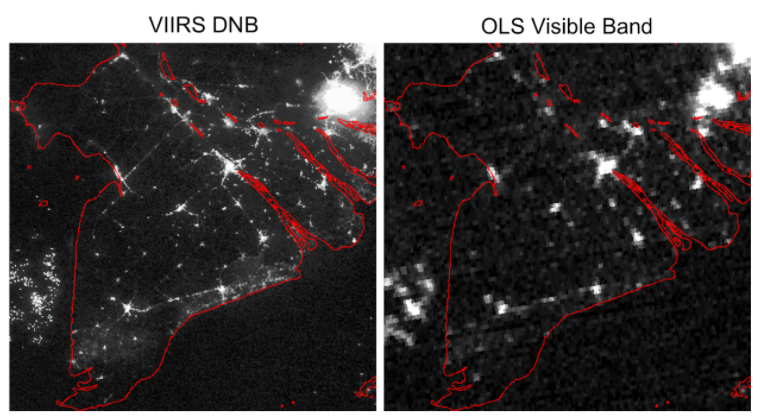
\includegraphics[width=260pt]{images/3.png}}
\caption{satellite}
\label{satellite1}
\end{figure}

The compared satellite pictures above show the different resolutions and details, and the result illustrates the VIIRS DNB's satellite 
data providing a clearer image.

In the AWS database, the folder includes massive files with NPP titles or names by date (Fig.~\ref{satellite2}). 

\begin{figure}[htbp]
    \centerline{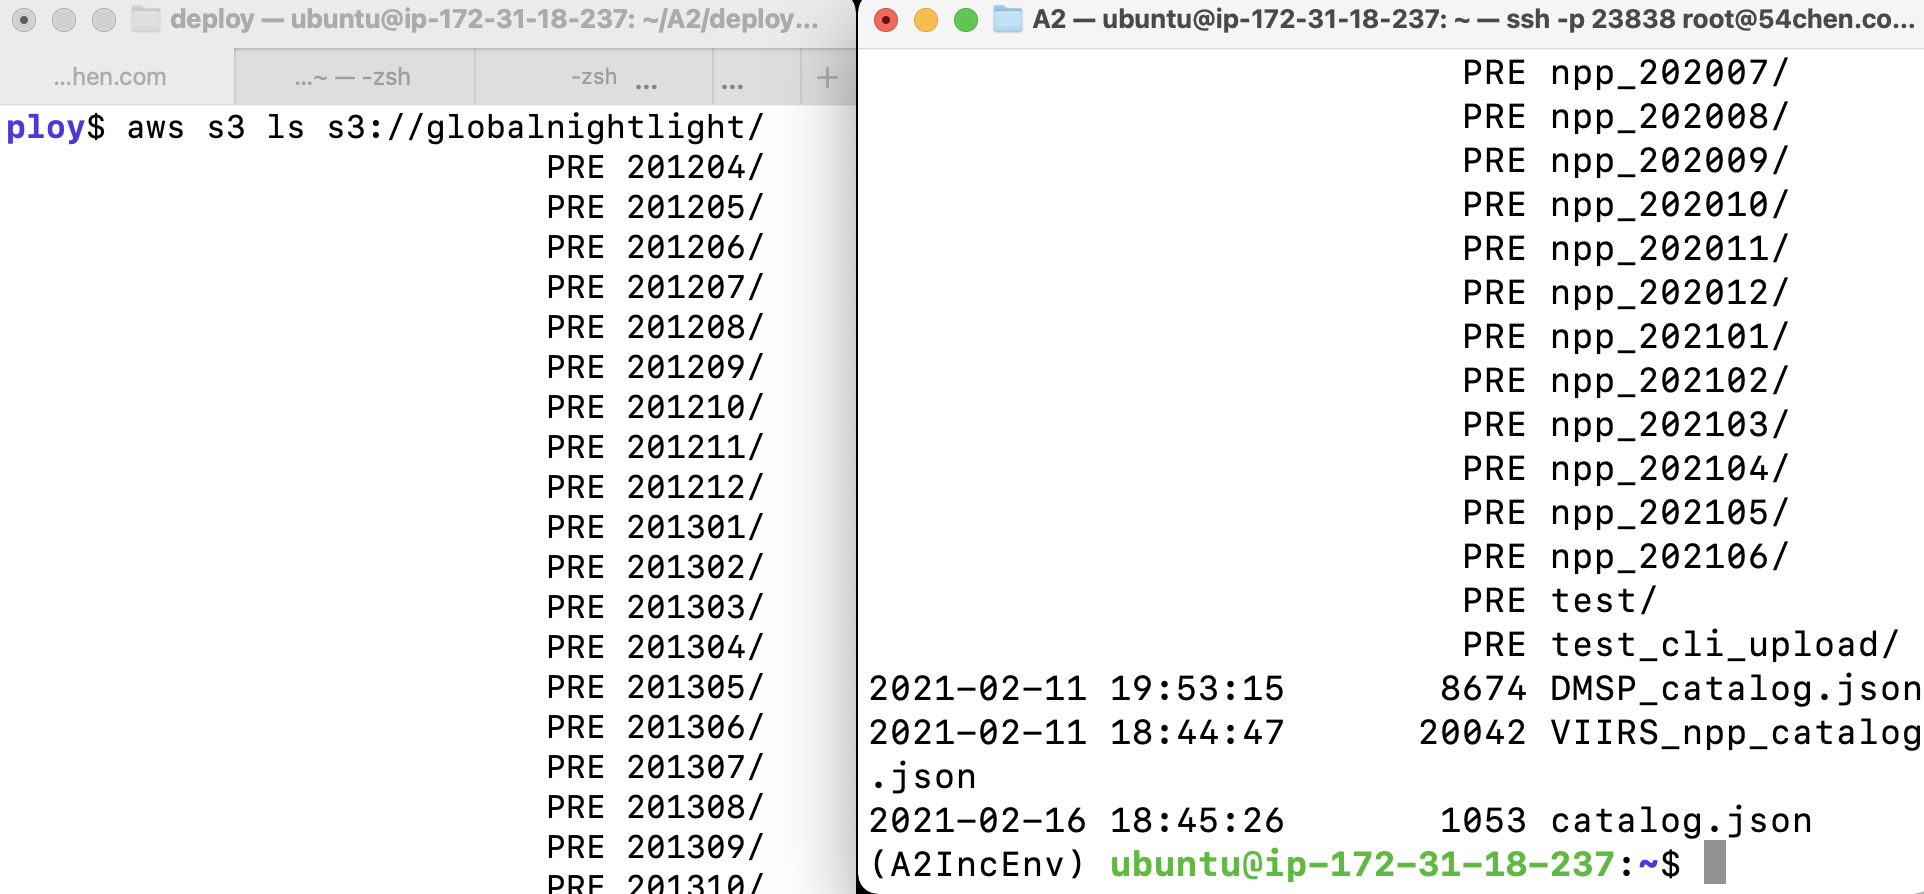
\includegraphics[width=260pt]{images/3.1.png}}
    \caption{files}
    \label{satellite2}
\end{figure}

The file named npp\_year and month is because of the data collection from VIIRS-DNB (the following DMSP-OLS sensor). 
It has some difference between DMSP.

The file example of data is called: SVDNB\_npp\_d201505\\04\_t1335358\_e1341162\_b18219\_c20150504194116381040\_\\noaa\_ops.rade9.co.tif. 
The file structure is:
Then there are lots details about what them are.
\begin{itemize}
    \item npp\_d20150504\_t1335358\_e1341162\_b18219
    \item npp = satellite ID
    \item d20150504 = start date of first scan in aggregate \\
    (2015/05/04)
    \item t1335358 = time of first scan (13:35:35.8)
    \item e1341162 = time of last scan (13:41:16.2)
    \item b18219 = orbit number of first scan
\end{itemize} 

The file:SVDNB\_npp\_d20150504\_t1335358\_e1341162\_b1\\
8219\_c20150504194116381040\_noaa\_ops

\begin{itemize}
    \item SVDNB = Day/Night Band SDR (all possible product IDs are listed below)
    \item npp\_d20150504\_t1335358\_e1341162\_b18219 = aggregate identifier
    \item C20150504194116381040 = creation date/time of SDR
    \item noaa = data origin
    \item ops = data domain
\end{itemize}

\subsubsection{Data structure}

The geospatial data be collected by satellites then all data will be stored in different types of formats or data types. 
In our project, there are two types of data formats, Raster file, and Vector file.

\paragraph{Raster file} 

The raster image is an image file format, which is composed of a pixel matrix composed of multiple grids, and each pixel 
contains an information value. The change of this information value will be reflected in different colors, positions, and 
sizes. The most commonly used raster data, such as aerial photographs, satellite images, or elevation surfaces. These 
oversized pictures are taken and collected through the reflection of the spectrum. Moreover, today's raster images are 
usually .BMP, .GIF, .JPEG, .PNG and .TIFF files (Katie, 2020, May 8). At present, almost all the images that the public 
can see on the Internet and the images taken by digital cameras are raster images. In our project, TIFF data files will 
become our research object.

\subparagraph{Use raster as the base map}

In GIS, raster data is usually used as the background display screen of other feature layers. Such layers are orthophotos, 
which not only provide additional information but also make map users more confident that the map layers are spatially 
aligned and represent actual objects. There are three main sources of such images, namely orthophoto aerial photography, 
orthophoto satellite images, and orthophoto scanned maps \cite{decsktop15:online}.

\subparagraph{Use raster as a surface map}

Rasters are usually used to represent data that changes continuously along the surface, such as rainfall, temperature, 
density, etc. The map draws the surface of the map through the continuously changing data of countless small grids. The 
continuous change of grid color reflects the change of a region at present or within a period \cite{decsktop15:online}.

\paragraph{Vector file}

In our project, the vector format data is not the main research object, but it is also a format that our team needs 
to understand. A vector data file is an image that can be scaled to any size without losing its quality and clarity. 
Changing the file has an advantage because its scaling depends on mathematical equations. This vector file is more 
flexible and has perfect image quality. Compared with Raster files, pixilation will not lose sharpness when zooming 
in, and raster graphics will be greatly affected to form sharp contrasts \cite{Thepaged34:online}.


\subsubsection{GeoTIFFs \& Cloud\-optimized geoTIFFs (COGs)}

Most of the files in the data on the AWS server are TIFF or TIF files, and these files are a file format used to 
store raster files. GeoTIFF is a TIFF file that follows specific standards used to construct metadata, such as geographic 
reference information, spatial extent, resolution, and number of layers.

Cloud Optimization GeoTIFFs (COG) is a cloud\-optimized file viewing, reading, and usage solution. The OGC GeoTIFF standard 
is the OGC implementation standard \cite{NASA23:online}. The files of GeoTIFFs are also GeoTIFF, and this data structured 
method allows users to query these files through Web services. However, this advantage allows users to query, analyze, visualize 
or download part of the COG file online without downloading the entire file. Such a database reading solution is also used by our team.

\subsubsection{Spatial\-Temporal Asset Catalog (STAC) standard}

The SpatioTemporal Asset Catalog (STAC) specification uses a common language to describe geospatial information to provide easier indexing and searching\cite{SpatioTe21:online}. "Space-time assets" is a kind of specific information to mark the file with the earth information data captured in different specific spaces and times. These data marked by the STAC specification will be published by the provider as a spatiotemporal asset catalog without the need to write new code collections or APIs. First of all, for providers, STAC is a standardized method, used to disclose spatiotemporal data collection assets when cataloging, and STAC is also a unified asset index method. Second, developers can build infrastructure to host, ingest, or manage spatial data collections, and can extend to custom domains. Finally, data consumers often have to build a unique pipeline for each different data set they use.


\subsection{Imagery processing in AWS}

The pictures in S3 are based on two essential formats, which are STAC and COG. The satellites generate them every day. 
The World Bank organized the global night lights project to store these files in S3. When it comes to dealing with the satellite 
imagery, Python has a lot of easy libraries for geospatial calculating. GDAL is the most useful one. 
It is integrated with Python very well, and is very good at reading and writing raster or vector geospatial file formats.
There are also some people sharing the source code of processing similar data \cite{Howtopro5:online}.


\begin{figure}[htbp]
    \centerline{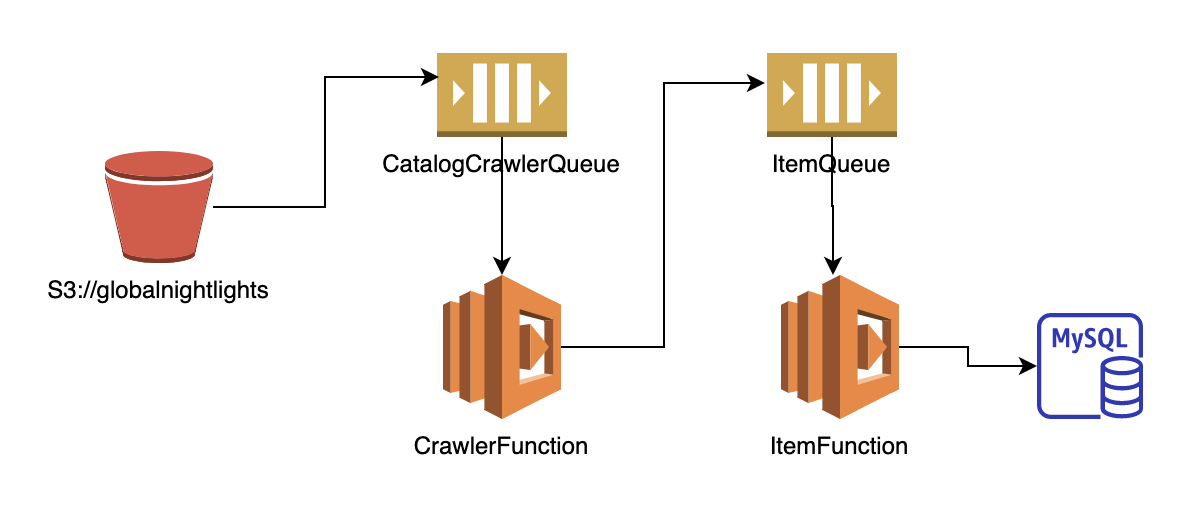
\includegraphics[width=260pt]{images/dataprocess.png}}
    \caption{Imagery processing in AWS}
    \label{fig4}
\end{figure}

Two Lambda functions are used for processing them, shown as Fig.~\ref{fig4}. The first one is to analyse the STAC protocol files. Boundary boxes can be found from a STAC file, therefore it is easy to index
all the imagery together by it and then to find the specific area by it. Root STAC file is the first file, which has all of the child links as Json files. 
Following the child links, there are the list items including the COG file URL. COG files are commonly too large to open directly. GDAL can open it easily and calculate radiance 
value in the file. In the second Lambda function, messages attached COG URL information exchanged by SQS service from the first Lambda function. Because of the complexity 
of GDAL computation, the second Lambda function is slower than the first one.

The second Lambda function is the main logic of data processing. First of all, choosing cities or areas is a deep issue. The original design was to show every administrative 
city. But the global administrative cities geospatial data is very difficult to get. Even though Global Administrative Unit Layers (GAUL) data is provided by Food and 
Agriculture Organization of the United Nation (FAO) \cite{GlobalAd98:online}, the format of these files still needs to research more. Therefore, the research areas were reduced 
to three specific areas, such as east of China, Middle East and New Zealand. Secondly, these three areas are defined in advance because they represent the areas of developed, 
developing and war. The radiance of these areas would show very different patterns. And reducing areas can help the function processing more quickly. Thirdly, calculating the 
radiance for every COG file is the core computation. There are intersection areas between the COG file and these three research places. And every pixel in the COG file stores 
a radiance value for this geospatial point. In the World Bank document, there are some special definitions about the value details, such as -999.3 means no-data value, -1.5 
means the beginning of the data range \cite{WorldBan13:online}. The value less than 3 could be disruption value. All of the numbers which are more than 3 could be the 
suitable value. In the end, all of the processed information is stored in RDS service. They are dates, boundary boxes, radiance, pixels and so on.

When it comes to the RDS, it is necessary to introduce the master and slave configuration. Because this global night lights data is stored in us-east-1 region and team members 
use ap-southeast-1 region, master database is installed at us-east-1 region which is closed to S3 data, and slave database is at another region. The cross-region RDS is 
provisioned by CloudFormation because there is a ready template. It has to be mentioned that the cross-region cost is not as cheap as other services.


\subsection{Testing}
Use Postman testing tool to test this website. The security testing of Web application system have:
1. Catalogue configuration
set catalogue correctly, every catalogue should have index.html page or main.html page.
2. Login
Our system does not apply first-registe-last-login method, so hence that we does not need to test
valid and invalid username and password, the functionality of third-party login is able to help
us authorized our credential, only need to do the manual testing.
3. Session
Testing whether web application system have restriction of timeout. In other word, user need to
login again after 15 seconds if they have not clicked anything in this webpage then the website
logout or not.
4. Log file
For ensuring web application service security, log file is really essential, it must be test whether
relative information is write into log file and whether information can be tracked or not.
5. Encryption
While using safe socket, we need to test whether the encryption is correct and check the integrity
of the information.
6. Security vulnerabilities
Server-side scripts often constitute security vulnerabilities, and these vulnerabilities are often exploited by hackers.
Therefore, it is also necessary to test the problem that scripts cannot be placed and edited on the server side without authorization.
7. Code legality test
Code legality testing mainly includes two parts:
*program code legality test.
*display code legality test.
8. Documentation test
Integrity accurency consistency suitable reasonable relativity testability.

\subsection{Project management}

Project management is also a big challenge in this special period. The Scrum development method was chosen from the first day because two members
had already experienced this method. This iterative approach towards the completion of a project can lead the team to success.

It is important that some tools let the team work like a native team. All of the team members are from China, but nobody knew each other before. 
So at the first day, the IM platform named Lark, which was widely used in the work place in China, was chosen by team members. Java is the first 
language in the team because team members are almost good at it. By Github, all of the code can be easily shared with members and easily taken 
control of its version. Remote cooperation is not an easy thing. Team members create an event for video meetings every day. At the same time, it 
is also an agile stand-up meeting every day. With the development and research process, some members have to stop to learn more things about the 
lack of relative knowledge. For example, none of the members are good at some key technologies, such as geospatial imagery processing, Vue, AWS usage. 
So the development plan was always disrupted because of learning. Thanks to the agile method, the entire project is not influenced too much by 
these disruptions. 

Because the members were not sharing the true space in the meeting room, the development atmosphere was a little bit strange. It is difficult to know 
every member's status. The enthusiasm of programming is of critical importance. Somebody went about their tasks with little enthusiasm, and the 
result of that part would be bad. At that time, the role of scrum master was very useful, it ensured the entire development schedule.

\section{Security Considerations}

Secruity is an important thing in programming. Although some services can enhance security, they are usually very expensive. For example, 
NAT can isolate the safer network. There are a lot of details contributing to the security together.

\subsection{Identity and Access management}

IAM is the first protection in this project. All of members' accounts opened the MFA login to ensure account security and avoided using the root user. 
Because these accounts are just used in code, they are disabled login with the password.

The team is divided into various different roles such as backend engineers, frontend engineers, 
testing, project managers, DBA. And all of the members would belong to one or more roles as Fig.~\ref{roles}. 

\begin{figure}[htbp]
    \centerline{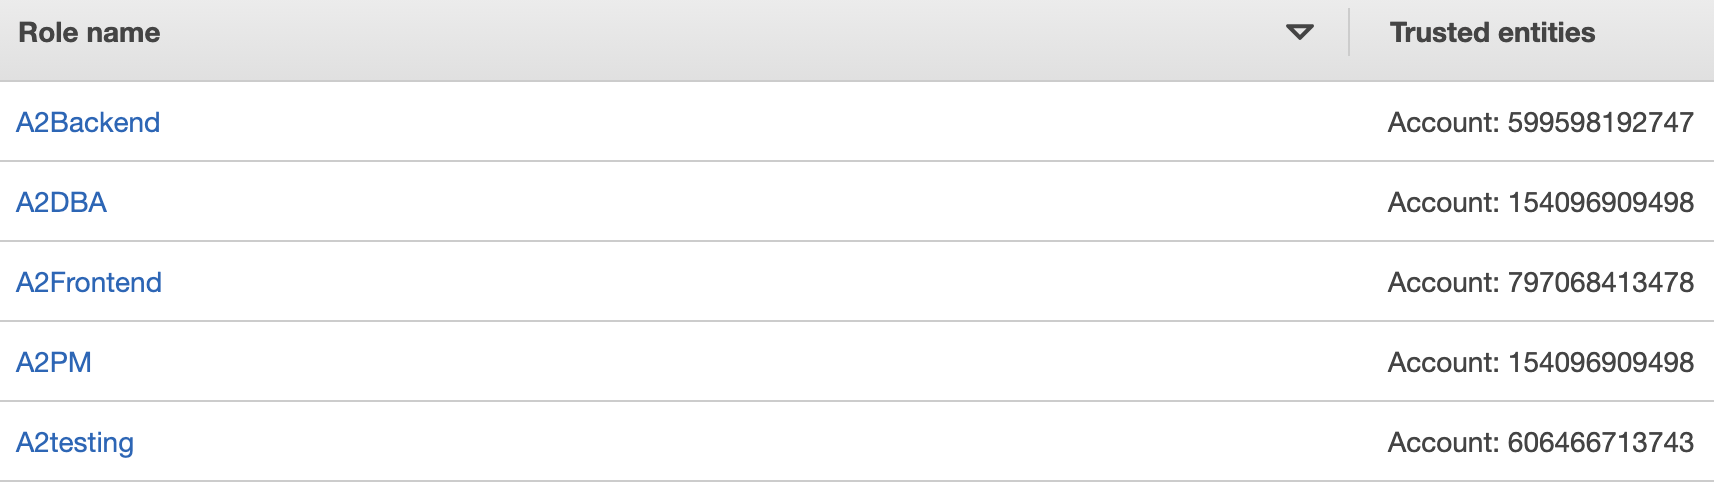
\includegraphics[width=260pt]{images/roles.png}}
    \caption{Roles in the team}
    \label{roles}
\end{figure}

Every role is attached to the least privileges which are \\ provided by AWS policies. As for project managers, the role of A2PM is an administrator role, and it is 
attached the AdministratorAccess policy. A2DBA is attached to AmazonRDSFullAccess policy, which is used by database administrator. A2Backend is attached 
AmazonRDSReadOnlyAccess and AmazonEC2ContainerServiceRole policies, which are used by backend engineers. A2Frontend is attached to AmazonEC2ContainerServiceforEC2Role 
policy and A2testing is attached to AmazonEC2ReadOnlyAccess policy. All the roles can protect the cloud environment and keep the least privilege. Practically, it is 
a little bit complicated for a small team, but it is useful especially when someone's credentials exposure at Github. And for the high privileges, only 
limited role can visit sensitive resources, for example, project managers can visit almost all of the resources.

Some roles are generated for the specific application. For example, there is a role named ec2callsecretsmanager. It is attached to the SecretsManagerReadWrite 
policy, which is used for an EC2 instance to visit the Secrets Manager service in AWS. It is a good method to hide the original password in the code and a 
convenient approach to get the privilege from one service to another service without any code.

For users, because the demo does not allow them to visit the visualisation without login, there are two roles. One is for guests, another is for login users. 
Guests' role is virtual. Guests can sign in with Gihub accounts. Github Oauth ensures authentication securely. Once they become authenticated users, 
all the visualisation can be shown, but they only have the read permission of the visualisation.


\subsection{Network}

To build a relatively safe network, there are 3 steps. The first step is to isolate public IP instances with others by subnet. In entire network design, 
ELB and deployment EC2 are the only two points that have a public IP address. This step can protect all of the services against attack even though some vulnerability 
would exist in some instances.

\begin{figure}[htbp]
    \centerline{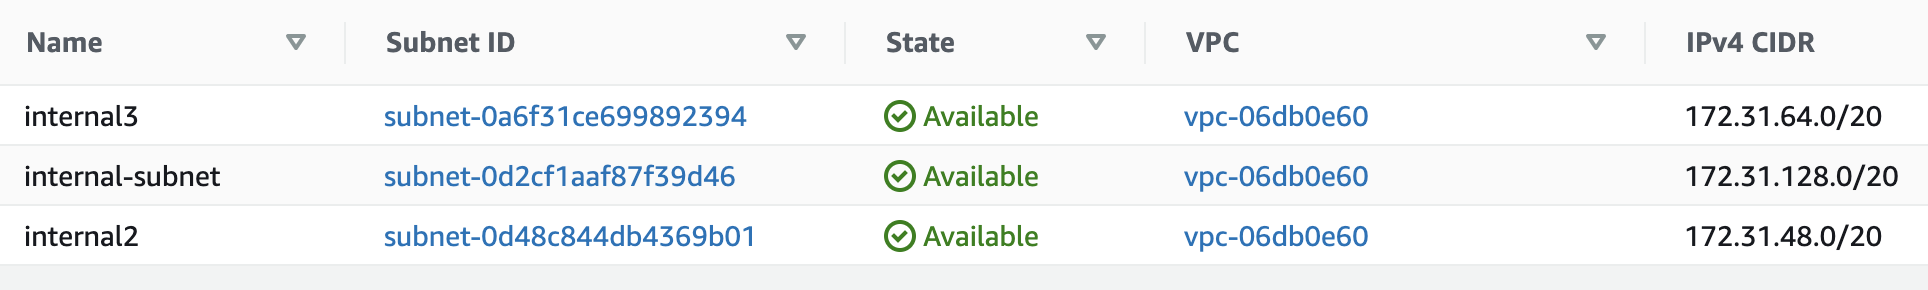
\includegraphics[width=260pt]{images/subnet.png}}
    \caption{Subnet}
    \label{subnet}
\end{figure}

The second step is the subnet design, which is shown as Fig.~\ref{subnet}. There are 3 different subnets used for services in different layers. And also, 
these subnet configurations help step 1 to isolate the public network environment. The subnets named Intranet2 and Intranet3 are isolated frontend 
instances. The benefit of this design is isolating the same functions into different partitions. When a part of the entire demo is hacked, it is easy 
to close this part to avoid more damage. The third subnet is the core which is connected with a database.

\begin{figure}[htbp]
    \centerline{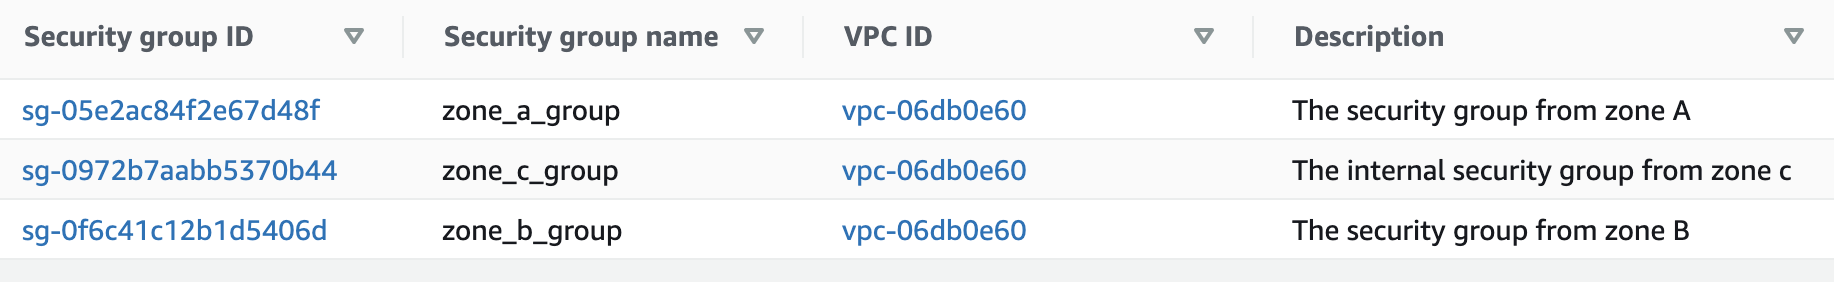
\includegraphics[width=260pt]{images/security.png}}
    \caption{Security groups}
    \label{Security}
\end{figure}

The last step is to configure the security groups for step 1 and 2. In this demo, 3 zones are divided into 3 subnets, which is shown as Fig.~\ref{Security}. The inbound 
rules of zone A and B allow port 80, which is the http service port connected by ELB in front of them. The zone C allows port 8080, which is the Tomcat 
service port connected by instances in zone A and B. And the outbound allows port 3306, which is the MySQL service port.

After these 3 steps, the network environment isolates all the services very well. It is fundamental protection.


\subsection{Data security}

Data in this demo is mainly in RDS MySQL, which is a kind of data in PaaS service model. There are two tables including "main" and "users". The table "main" 
stores all of the data needed by the visualisation. The another one stores all of the user's information. There are some steps to ensure data security.

\subsubsection{Step 1. Identification \& Category}

S3 public data is also used in this demo. Because everyone can read this data, there is no special permission setting in this demo. RDS MySQL provided authentication 
by itself. The user and password can be used for the RDS MySQL. Moreover, the password is automatically generated and rotated by a Lambda function. That is a  
very good practical design in AWS.

For classification, all the data is divided into three kinds of data including public original data, imagery data after processing, user data. The most sensitive 
data is the third one. 

\subsubsection{Step 2. High level policy}

Because the user data stored in RDS is the highly sensitive data in this demo, only Java instances are allowed to visit it. And the entitlement matrix 
is shown as Fig.~\ref{matrix}.

\begin{figure}[htbp]
    \centerline{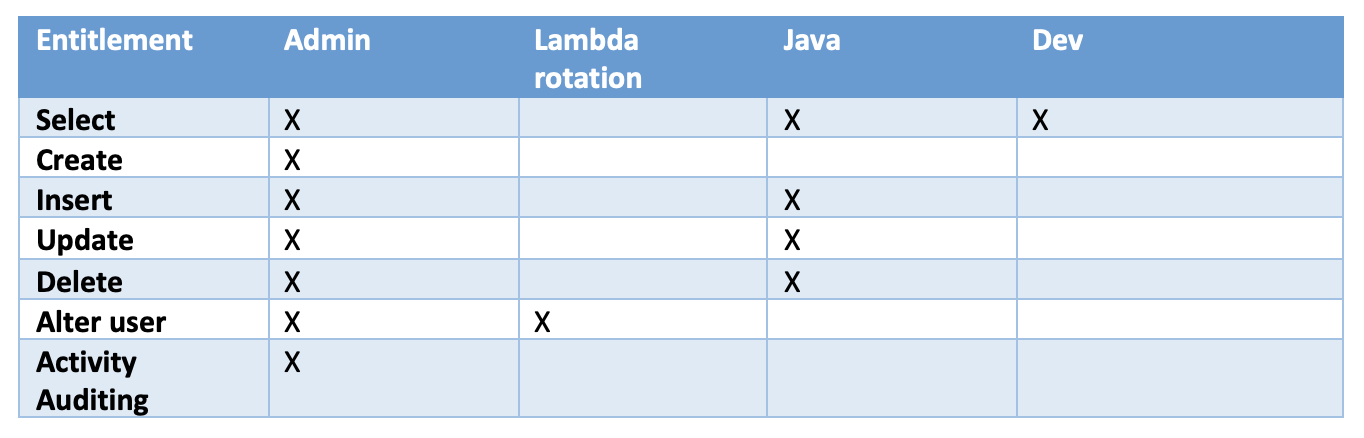
\includegraphics[width=260pt]{images/matrix.png}}
    \caption{Entitlement matrix}
    \label{matrix}
\end{figure}

There are some accurate permission control methods provided by MySQL. The entitlement matrix is made by the MySQL privileges. Admin account is the supper administrator 
which is managed by the project manager role. It is responsible for the management of database creating and auditing. And also, resource based policies provided 
by IAM also give basic data security, which is the role named AWSServiceRoleForRDS allowing the EC2 instance to visit RDS. At the application layer, the guest role 
has no permission to read the user data. As for the data sharing layer, the user data has no need to be shared, so it does not take it into consideration. At the auditing layer, 
project manager is responsible for the daily work of account based auditing.

\subsubsection{Step 3. Encryption}

From the entrance, https is the first consideration of security. Https protocol uses TLS, which is a kind of asymmetric encryption, and when the secret key is exchanged, 
it uses symmetric encryption to transfer data. All of the data can be protected by it. Because this demo has no http domain name, https has not configured.

For the data at rest encryption, RDS can enable the encryption when the database is created. And the key is stored in KMS. It is the cloud handles encryption. Actually, it 
is not enabled in this demo because there is not any extremely sensitive data like passwords and so on.

For the data in motion encryption, https is the most useful method between users and this demo. And also, Github Oauth provides a safe method to identify the user. When 
users follow the Github login url to get the one time code, they send the code to this demo, and this demo will visit Github api with the code by the Oauth2 protocol. All the 
processes are protected by Github design. After the identifying of the user, a session could be stored in the server, and generating a new encrypted cookie named JSEESIONID. With is 
cookie in every following visit, this demo can ensure user login status.

\subsubsection{Step 4. What is more}

Data in this project is not so highly sensitive. For example, S3 data is public for everyone, the calculating data is also public for every authenticated user. Only user 
information is private data. Reasonable security is good for the performance of an internet demo. Generally, after the above steps, the data 
security would be sufficient, but the devil is in detail, every step needs to be cautious to implement, and make sure that performance does not degrade too much.

\section{Actual AWS expenditure}

Totally spend 60\$. The imagery processing accounted for 33 percent. EC2 accounted for 33 percent. RDS accounted for 17 percent. Others accounted for 17 percent, including NAT.

\begin{itemize}
    \item Lambda: 20\$
    \item EC2:20\$
    \item RDS:10\$
    \item NAT:10\$
\end{itemize}

\section{Team members and individual contribution within the team}

\subsection{Zhen Chen}
\textbf{Role and Tasks:} PM, BE, DevOps. Scrum master. Designed the entire backend architecture. 
    Implemented all the imagery processing Python code. Implemented all the deployment code. 
    Implemented part of the backend Java code. 

\textbf{Writing contribution includs:} The previous 8 paragraphs of solution summary, and F, G, H, I, J 
    subsections in it. The A, E, G subsections of proposed solution. The section of security 
    Considerations. The section of actual AWS expenditure.

\subsection{Huajie Xu} 
\textbf{Role and Tasks:} FE. Designed and implemented the entire fronted part of solution. Participated in frontend \& backend debugging.

\textbf{Writing contribution includs:} The D, E subsections of solution summary. The B subsections of proposed solution.

\subsection{Shengzhu Wang}
\textbf{Role and Tasks:} BE. Implemented part of the backend Java code. 
 
\textbf{Writing contribution includs:} Quit the team early without participating in writing.

\subsection{SiXiang Xiong}
\textbf{Role and Tasks:} BE, Testing.

From my perspective, I have study many methods of writing user login and third party login,
finally learning how to implement the third party login with github as for our website,
usually we use OAuth2, springboot, then select java to develop, in this project, I help to test
this website though postman.

\textbf{Writing contribution includs:} The K subsection of solution summary. The C, F subsections of proposed solution.

\subsection{Wenjie Tong} 
\textbf{Role and Tasks:} UI designer,Data Researcher, Testing.

    In my part of this project, I am playing a role of UI designer,Data Researcher and function 
    tester. 
    Implementing part of the contribution:
    UI desgin is based on functions to develop the web pages.
    Data reseach regarding with World Bank Light Every Light doucument,and I have done further 
    study to understand the related knowledge about DSMP-OLS and VIISR-DNB data.
    I will take a part of testing task to ensure the functionality of our project.

\textbf{Writing contribution includs:} The A, B, C subsections of solution summary. 
    The D subsection of proposed solution.
  
\printbibliography

\end{document}
